%Version 3.1 December 2024
% See section 11 of the User Manual for version history
%
%%%%%%%%%%%%%%%%%%%%%%%%%%%%%%%%%%%%%%%%%%%%%%%%%%%%%%%%%%%%%%%%%%%%%%
%%                                                                 %%
%% Please do not use \input{...} to include other tex files.       %%
%% Submit your LaTeX manuscript as one .tex document.              %%
%%                                                                 %%
%% All additional figures and files should be attached             %%
%% separately and not embedded in the \TeX\ document itself.       %%
%%                                                                 %%
%%%%%%%%%%%%%%%%%%%%%%%%%%%%%%%%%%%%%%%%%%%%%%%%%%%%%%%%%%%%%%%%%%%%%

%%\documentclass[referee,sn-basic]{sn-jnl}% referee option is meant for double line spacing

%%=======================================================%%
%% to print line numbers in the margin use lineno option %%
%%=======================================================%%

%%\documentclass[lineno,pdflatex,sn-basic]{sn-jnl}% Basic Springer Nature Reference Style/Chemistry Reference Style

%%=========================================================================================%%
%% the documentclass is set to pdflatex as default. You can delete it if not appropriate.  %%
%%=========================================================================================%%

%%\document parenthesis. class[sn-basic]{sn-jnl}% Basic Springer Nature Reference Style/Chemistry Reference Style

%%Note: the following reference styles support Namedate and Numbered referencing. By default the style follows the most common style. To switch between the options you can add or remove �Numbered� in the optional
%%The option is available for: sn-basic.bst, sn-chicago.bst%  
 
%%\documentclass[pdflatex,sn-nature]{sn-jnl}% Style for submissions to Nature Portfolio journals
%%\documentclass[pdflatex,sn-basic]{sn-jnl}% Basic Springer Nature Reference Style/Chemistry Reference Style
\documentclass[pdflatex,sn-mathphys-num]{sn-jnl}% Math and Physical Sciences Numbered Reference Style
%%\documentclass[pdflatex,sn-mathphys-ay]{sn-jnl}% Math and Physical Sciences Author Year Reference Style
%%\documentclass[pdflatex,sn-aps]{sn-jnl}% American Physical Society (APS) Reference Style
%%\documentclass[pdflatex,sn-vancouver-num]{sn-jnl}% Vancouver Numbered Reference Style
%%\documentclass[pdflatex,sn-vancouver-ay]{sn-jnl}% Vancouver Author Year Reference Style
%%\documentclass[pdflatex,sn-apa]{sn-jnl}% APA Reference Style
%%\documentclass[pdflatex,sn-chicago]{sn-jnl}% Chicago-based Humanities Reference Style

%%%% Standard Packages
%%<additional latex packages if required can be included here>

\usepackage{graphicx}%
\usepackage{multirow}%
\usepackage{amsmath,amssymb,amsfonts}%
\usepackage{amsthm}%
\usepackage{mathrsfs}%
\usepackage[title]{appendix}%
\usepackage{xcolor}%
\usepackage{textcomp}%
\usepackage{manyfoot}%
\usepackage{booktabs}%
\usepackage{algorithm}%
\usepackage{algorithmicx}%
\usepackage{algpseudocode}%{\tiny }
\usepackage{listings}%
\usepackage{tikz}%
%%%%

%% as per the requirement new theorem styles can be included as shown below
\theoremstyle{thmstyleone}%
\newtheorem{theorem}{Theorem}%  meant for continuous numbers
\newtheorem{corollary}{Corollary}%
\newtheorem{lemma}{Lemma}%
%%\newtheorem{theorem}{Theorem}[section]% meant for sectionwise numbers
%% optional argument [theorem] produces theorem numbering sequence instead of independent numbers for Proposition
\newtheorem{proposition}[theorem]{Proposition}% 
%%\newtheorem{proposition}{Proposition}% to get separate numbers for theorem and proposition etc.

\theoremstyle{thmstyletwo}%
\newtheorem{example}{Example}%
\newtheorem{remark}{Remark}%

\theoremstyle{thmstylethree}%
\newtheorem{definition}{Definition}%

\raggedbottom
%%\unnumbered% uncomment this for unnumbered level heads

\begin{document}

\title[Article Title]{Approximation Algorithms for the Robust Selection Problem: Primal and Primal-Dual Rounding}

%%=============================================================%%
%% GivenName	-> \fnm{Joergen W.}
%% Particle	-> \spfx{van der} -> surname prefix
%% FamilyName	-> \sur{Ploeg}
%% Suffix	-> \sfx{IV}
%% \author*[1,2]{\fnm{Joergen W.} \spfx{van der} \sur{Ploeg} 
%%  \sfx{IV}}\email{iauthor@gmail.com}
%%=============================================================%%

\author*[1]{\fnm{Trajana} \sur{Erlenberg}}\email{Trajana.Erlenberg@uni-passau.de}

\author[1]{\fnm{Marc} \sur{Goerigk}}\email{Marc.Goerigk@uni-passau.de}

\author[1]{\fnm{Dorothee} \sur{Henke}}\email{Dorothee.Henke@uni-passau.de}

\affil[1]{\orgdiv{Business Decisions and Data Science}, \orgname{University of Passau}, \orgaddress{\street{Dr.-Hans-Kapfinger-Str. 30}, \city{Passau}, \postcode{94032}, \state{Bavaria}, \country{Germany}}}

\abstract{As robust combinatorial problems are often computationally hard, finding approximation algorithms is of great interest to researchers in the field. The \textsc{MinMax Selection} problem is a frequently studied problem in this context, with the best known approximation result of \(O(\log k/\log\log k)\) achieved via dependent randomized rounding. We provide two additional approximation algorithms for this problem. Firstly, a primal rounding procedure, which, despite its simplicity, admits a \(\min\{k, n - p + 1\}\)- approximation guarantee, improving upon known bounds in specific parameter regimes. Secondly, a primal-dual rounding procedure, admitting a \(k\)-approximation, while being a generalization of the well known midpoint method. Primal-dual rounding can be improved by first solving a linear program to find an optimal representative weight vector and then applying the algorithm using this vector. For the \textsc{MaxMin Selection} problem, we establish inapproximability for unbounded \(k\). Computational experiments show that the primal rounding approach provides particularly good practical solutions compared to primal-dual rounding and representative scenario approaches, such as the midpoint method and the worst-case-per-item method.}

\keywords{Robust optimization, Combinatorial optimization, Approximation algorithms, Selection problem, Primal rounding, Primal-dual rounding}

%%\pacs[JEL Classification]{D8, H51}

%%\pacs[MSC Classification]{35A01, 65L10, 65L12, 65L20, 65L70}

\maketitle

\section{Introduction}
\label{intro}

In the context of decision-making, it is often required to make an informed choice which leads to an advantageous outcome or meets a pre-specified goal \cite{Nocedal2006}. The field of optimization is concerned with modeling such problems in mathematical terms and solving them as best as possible. However, classical nominal models assume fixed, known parameters, while real-world decision-making situations are often subject to some degree of uncertainty (e.g. in the variables or the environment) \cite{Li2024}. When nominal models are exposed to even a small degree of uncertainty, the results often become infeasible \cite{BenTal2009}. To find favorable solutions under uncertain conditions, one can use the concept of robust optimization. Unlike stochastic optimization, this approach does not rely on probability distributions, making it especially suitable for high-impact, low-probability events \cite{Aissi2009}. At the same time, adding uncertainty to a nominal optimization problem can significantly increase its complexity \cite{Kasperski2016}, making the development of approximation algorithms particularly important in the field of robust optimization.

For an overview on the topics of robust combinatorial optimization and approximation algorithms, we refer to the books \cite{Goerigk2024} and \cite{Williamson2011}, respectively.

This paper focuses on the \textsc{Selection} problem, which is a fundamental combinatorial problem, frequently studied in robust optimization due to its structural simplicity.
Given a set of $n \in \mathbb{Z}_{>0}$ items, each with a non-negative cost $c_i \in \mathbb{R}_{\ge0}$, and an integer $p \in \mathbb{Z}_{\ge0}$ \((p \leq n)\), select exactly \(p\) items such that the total cost is minimized. Note that the cases \(p = 0\) and \(p = n\) are trivial. The problem is formally defined as follows:
\[
\min \left\{ \sum_{i \in [n]} c_i x_i : \sum_{i \in [n]} x_i = p,\; x \in \{0,1\}^n \right\}.
\]
The \textsc{Selection} problem in its basic deterministic form is solvable in (weakly) polynomial time using a linear program (LP), since the coefficient matrix is totally unimodular by the Ghouila-Houri criterion. An even better performance can be achieved either through simple sorting with a complexity of \(O(n \log n)\) or via more sophisticated methods based on median-finding techniques, which achieve a complexity of \(O(n)\). The \textsc{Selection} problem can also be seen as a matroid problem, implying that some greedy algorithm always yields an optimal solution \cite{Goerigk2024, Papadimitriou1998}. Note that the \textsc{Selection} problem is a special case of several combinatorial problems, including min-knapsack, minimum assignment, minimum matroid base and resource allocation \cite{Kasperski2013}.

To add robustness to an optimization problem, we need to specify an uncertainty set \( \mathcal{U} \subseteq \mathbb{R}^n_{\ge0}\) (e.g. discrete, interval, budgeted, polytopal) representing all possible realizations of an uncertain parameter. This paper concentrates on discrete uncertainty, using a finite set of \(k\) explicitly listed cost scenarios: \( \mathcal{U} = \{ c^{1}, c^{2}, \dots, c^{k} \} \). This set is especially relevant to model a limited number of well-defined future events, such as market reactions or public policy decisions. Further, we need a decision criterion (e.g. min-max, min-max regret, recoverable, two-stage), to define how a solution is determined. Here, we use the min-max (and max-min) criterion. The goal is to minimize the worst-case cost across all scenarios in \( \mathcal{U} \). It is the most classical and conservative criterion and is useful in situations, where decisions are non-repetitive and errors may have severe, irreversible consequences \cite{Aissi2009, Goerigk2024}. Let \(k \in \mathbb{Z}_{> 0}\) be the number of cost scenarios and $\mathcal{X} \subseteq \{0, 1\}^n$ be the set of feasible solutions. The \textsc{MinMax Selection} problem under discrete uncertainty is formulated as follows:
\[
\min_{x \in \mathcal{X}} \; \max_{c \in \mathcal{U}} \sum_{i \in [n]} c_i x_i \qquad
\text{with} \quad \mathcal{X} = \left\{ x \in \{0,1\}^n \;:\; \sum_{i \in [n]} x_i = p \right\}, \quad
\mathcal{U} = \left\{ c^{1}, c^{2}, \dots, c^{k} \right\}
\]
For the case of a single cost scenario, the robust \textsc{Selection} problem coincides with the nominal \textsc{Selection} problem and is thus solvable in polynomial time \cite{Goerigk2024}.
Using the epigraph reformulation, we introduce a continuous variable \( z \in \mathbb{R}_{\ge 0} \) that represents an upper bound on the scenario costs. In the optimal solution, \( z \) equals the maximum scenario cost. This yields the following compact MILP formulation:
\begin{alignat}{3}
	\label{eq:minmax_lp}
	\min \quad & z \\
	\text{s.t.}\quad
	& \sum_{i=1}^{n} x_i = p & \quad & \label{eq:minmax_lp:card}\\
	& \sum_{i=1}^{n} c^{s}_{i}\, x_i \le z && \forall s \in [k] \label{eq:minmax_lp:scenario} \\
	& x_i \in \{0,1\} && \forall i \in [n] \label{eq:minmax_lp:integrality} \\
	& z \in \mathbb{R}_{\ge 0}
\end{alignat}
For a constant number of scenarios \(k\), the \textsc{MinMax Selection} problem with discrete uncertainty, in the literature also referred to as min-max selecting items, is weakly NP-hard even if \(k = 2\) \cite{Averbakh2001}. It admits a pseudopolynomial-time algorithm and even a fully polynomial-time approximation scheme (FPTAS) \cite{Goerigk2024}. For details on the two main approaches for designing FPTAS for several min-max combinatorial optimization problems we refer to \cite{Papadimitriou2000, Aissi2006}.

In contrast, when the number of scenarios \(k\) is part of the input (i.e., \(k\) is unbounded), the \textsc{MinMax Selection} problem with discrete uncertainty is strongly NP-hard and not approximable within $2 - \epsilon$ for any $\epsilon > 0$ unless P = NP \cite{Kasperski2009}. It is further shown that the problem cannot be approximated within any constant factor unless P = NP \cite{Kasperski2013}. Over the years the problem has been intensively studied and several heuristics and approximation methods have been developed and tested: 

An intuitive heuristic is the solve-each-scenario idea: solve \textsc{Selection} for all $s \in [k]$ and pick the best solution. Since solutions optimized for one scenario may perform arbitrarily poorly in others, this gives no guarantee for min-max problems \cite{Aissi2009, Goerigk2024}.

A simple deterministic approximation is the midpoint method. The idea is to replace the scenario-dependent costs $c^s_i$ by their average over all scenarios, i.e., $\bar{c}_i = \tfrac{1}{k}\sum_{s=1}^k c^s_i$ for each item $i \in [n]$. This is a $k$-approximation for the original robust problem. Note that this does not hold for the max-min version \cite{Aissi2009, Kasperski2013}.

Another simple deterministic approximation approach is the worst-case-per-item method (WCPI): the costs $c^s_i$ of each item $i \in [n]$ are replaced by their worst-case value $c'_i = \max_{s \in [k]} c^s_i$. This constitutes a tight $k$-approximation for the original problem, which does again not hold for the max-min version \cite{Aissi2009, Goerigk2024}.\footnote{A more general perspective on approximation methods based on a single representative scenario is provided by \cite{Goerigk2019}. Scenario aggregation can improve both the midpoint and the WCPI method, yielding a polynomial-time $(\varepsilon k)$-approximation for any fixed $\varepsilon > 0$ \cite{Chassein2018}.}

The first more complex algorithm, based on randomized rounding, was presented in \cite{Kasperski2009}. It uses a strengthened LP relaxation (denoted as $LP(W)$), which only considers items whose costs in all scenarios are at most~\(W\). Under mild assumptions, the procedure returns an \(O(\ln k)\)-approximate solution with a certain probability.
These results are strengthened in \cite{Kasperski2013} by slightly modifying the procedure, which allows the algorithm to succeed in a single run and later enables its derandomization, so it always returns a feasible $O(\ln k)$-approximate solution in polynomial time.

The asymptotically strongest result is given in \cite{Doerr2013} with a deterministic \(O(\log k/\log\log k)\)-approximation, based on the same LP formulation as \cite{Kasperski2009}. 
From the fractional solution, dependent randomized rounding is applied and then derandomized. The approach runs in polynomial time in the RAM model of computation. They also prove an integrality gap of \(\Omega(\log k/\log\log k)\) for the same LP formulation, implying that approaches based solely on this LP cannot asymptotically beat \(\Theta(\log k/\log\log k)\).

In this work, we also consider the \textsc{MaxMin Selection} problem, which focuses on maximizing the minimum value over all scenarios \cite{Goerigk2024}: \(\max_{x \in \mathcal{X}} \min_{c \in \mathcal{U}} \sum_{i \in [n] } c_i x_i\). Maximization problems typically differ significantly from their minimization counterparts and often do not admit analogous approximation guarantees \cite{Aissi2009}. To the best of our knowledge, the computational complexity and approximability of the \textsc{MaxMin Selection} problem have not yet been explicitly investigated in the literature. 

Table \ref{summary} summarizes known and new approximation results for robust \textsc{Selection}.

%\begin{table}[h]
%	\caption{Summary of approximation and hardness results for robust \textsc{Selection}}\label{tab1}%
%	\begin{tabular}{@{}llll@{}}
%		\toprule
%		\textbf{Problem} & \textbf{Complexity}  & \textbf{Algorithm} &\textbf{Approximation} \\
%		\midrule
%		\textsc{MinMax S.}, & Weakly NP-hard    & FPTAS  & (1 + $\varepsilon$)-approx. \cite{Averbakh2001}  \\
%		\medskip
%		const. $k$ &&&\\
%		\textsc{MinMax S.},    & Strongly NP-hard   & Midpoint \&    &  $k$-approx. \cite{Aissi2009}  \\
%		\medskip
%		 unbounded $k$&&Worst-case-per-item&\\
%		 \medskip
%		 &   & Scenario aggregation	& $(\varepsilon k)$-approx. \cite{Chassein2018}   \\
%		 \medskip
%		 &   & Rand.\ rounding & $O(\ln k)$-approx. \cite{Kasperski2013} \\
%		 \medskip
%		 &   & Dep.\ rounding	& $O(\tfrac{\log k}{\log\log k})$-approx. \cite{Doerr2013}  \\
%		 \medskip
%		 &   &  Primal rounding & $\min\{k,n-p+1\}$-approx. (Cor.~\ref{cor:min_combined_bound}) \\
%		\medskip
%		 &   & Primal-dual rounding	& $1/\beta_{\min}$ (=$k$ uniform) (Thm.~\ref{thm:primaldual_priori})  \\
%		\textsc{MaxMin S.},    & Strongly NP-hard    & -  & Inapproximable (Thm.~\ref{thm:maxmin_inapprox_unbounded_k})  \\
%		unbounded $k$ &&&\\
%		\botrule
%	\end{tabular}
%\end{table}

\begin{table}[h]
	\caption{Summary of approximation and hardness results for robust \textsc{Selection}}
	\label{summary}
	\centering
	\begin{tabular}{@{}llll@{}}
		\toprule
		\textbf{Problem} & \textbf{Complexity} & \textbf{Algorithm} & \textbf{Approximation} \\
		\midrule
		\textsc{MinMax S.}, const.\ $k$ & wNP-hard & FPTAS & $(1+\varepsilon)$-appr.\ \cite{Averbakh2001} \\
		\addlinespace[2pt]
		\textsc{MinMax S.}, unb. $k$ & sNP-hard & Midpoint \& WCPI & $k$-appr.\ \cite{Aissi2009} \\
		\addlinespace[1pt]
		&  & Scenario aggregation & $(\varepsilon k)$-appr.\ \cite{Chassein2018} \\
		&  & Rand.\ rounding & $O(\ln k)$-appr.\ \cite{Kasperski2013} \\
		&  & Dep.\ rounding & $O(\tfrac{\log k}{\log\log k})$-appr.\ \cite{Doerr2013} \\
		&  & Primal rounding & $\min\{k,n-p+1\}$-appr.\ (Cor.~\ref{cor:min_combined_bound}) \\
		&  & Primal-dual rounding & $k$-appr. (Thm.~\ref{thm:primaldual_priori}) \\
		\addlinespace[2pt]
		\textsc{MaxMin S.}, unb. $k$ & sNP-hard & -- & Inapproximable (Thm.~\ref{thm:maxmin_inapprox_unbounded_k}) \\
		\botrule
	\end{tabular}
\end{table}
\noindent
The remainder of this paper is structured as follows. In Section~\ref{primal}, we introduce a primal rounding algorithm for \textsc{MinMax Selection} and derive its a priori guarantees as well as tightness and integrality-gap results for the underlying LP. In Section~\ref{primal-dual}, we present a primal-dual rounding approach, analyze its guarantee, and improve it by using a preceding representative-scenario LP. Section~\ref{inapprox} studies the \textsc{MaxMin Selection} variant and proves inapproximability for unbounded $k$. Finally, Section~\ref{exp} reports experiments comparing the methods, and Section~\ref{concl} concludes the paper.

\section{Primal rounding under the min-max criterion}
\label{primal}

In this section, we consider the \textsc{MinMax Selection} problem under discrete uncertainty, as formally defined in formulation~\eqref{eq:minmax_lp}. We propose a simple primal rounding approach that provides an efficient approximation. 
Algorithm \ref{alg:primal-rounding-minmax} solves the LP relaxation ($x_i \in [0,1]$) and obtains an optimal solution $x^*$, then deterministically rounds the $p$ largest entries of $x^*$ to produce a binary solution.
\begin{algorithm}[H]
	\caption{Primal rounding for \textsc{MinMax Selection}}
	\label{alg:primal-rounding-minmax}
	\begin{algorithmic}[1]
		\State Solve the LP relaxation:
		\[
		\min \; z \quad \text{s.t.} \quad \sum_{i=1}^n x_i = p, \quad \sum_{i=1}^n c^s_i x_i \le z \; \forall s \in [k], \quad x_i \in [0,1]
		\]
		\State Let $x^* \in [0,1]^n$ be an optimal fractional solution
		\State Sort the components of $x^*$ in non-increasing order
		\State Select the indices $i_1, \dots, i_p$ corresponding to the $p$ largest components of $x^*$
		\State Set $\hat x_{i} \gets 1$ for all $i \in \{i_1,\dots,i_p\}$ and all other components to $0$\\
		\Return $\hat{x}$
	\end{algorithmic}
\end{algorithm}

\noindent
The overall runtime of the primal rounding algorithm has three main components: solving the LP, sorting the fractional solution vector \(x^*\) and selecting the \(p\) largest components. The LP relaxation of the robust \textsc{Selection} problem can be solved in polynomial time using standard LP solvers such as the interior-point method \cite{Karmarkar1984}.
The sorting requires \(O(n \log n)\) time, followed by a linear-time selection step. Since all individual steps are polynomial in the input size, the entire algorithm runs in polynomial time.\\

\noindent
We now establish an a priori guarantee for Algorithm~\ref{alg:primal-rounding-minmax}.
\begin{lemma}
	\label{lem:min-component}
	Let \( p \in [n] \) and let \( x = (x_1, \dots, x_n) \in \mathbb{R}^n \) be a vector such that
	\[
	x_1 \ge x_2 \ge \dots \ge x_n, \quad x_i \in [0,1] \text{ for all } i \in [n], \quad \text{and} \quad \sum_{i=1}^n x_i = p.
	\]
	Then
	\[
	x_p \ge \frac{1}{n - p + 1}.
	\]
	\begin{proof}
		Since \( x_i \le 1 \) for all \( i \in [n] \), the sum of the first \( p - 1 \) components satisfies
		\[
		\sum_{i=1}^{p-1} x_i \le p - 1.
		\]
		We split the total sum as
		\[
		\sum_{i=1}^n x_i = \sum_{i=1}^{p-1} x_i + \sum_{i=p}^n x_i = p,
		\]
		which implies
		\[
		\sum_{i=p}^n x_i = p - \sum_{i=1}^{p-1} x_i \ge p - (p - 1) = 1.
		\]
		Since the vector is sorted in non-increasing order, we have \( x_p \ge x_{p+1} \ge \dots \ge x_n \), so the average of the components \( x_p, \dots, x_n \) is at most \( x_p \). Therefore,
		\[
		\frac{1}{n - p + 1} \sum_{i=p}^n x_i \le x_p 
		\quad \Rightarrow \quad 
		\sum_{i=p}^n x_i \le (n - p + 1) \cdot x_p.
		\]
		Combining both bounds yields
		\[
		(n - p + 1) \cdot x_p \ge 1 \quad \Rightarrow \quad x_p \ge \frac{1}{n - p + 1}.
		\]
	\end{proof}
\end{lemma}
\begin{lemma}
	\label{thm:frac_bound}
	Let $x^* \in [0,1]^n$ be a basic optimal solution of the LP relaxation of the \textsc{MinMax Selection} problem with $k$ scenarios. Then $x^*$ contains at most $k$ fractional variables.
	\begin{proof}
		To analyze the LP, we rewrite the original LP from formulation~\eqref{eq:minmax_lp} in standard form and introduce slack variables:
		\begin{itemize}
			\item Introducing slack variables $y_s \ge 0$ for each scenario constraint: \(\sum_{i=1}^n c^s_i x_i + y_s = z \quad \forall s \in [k]
			\)
			\item Modeling the upper bound $x_i \le 1$ with slack variables $d_i \ge 0$: 
			\(
			x_i + d_i = 1 \quad \forall i \in [n]
			\)
			\item The lower bounds $x_i \ge 0$ are implicitly satisfied in the standard LP form.
		\end{itemize}
		The resulting LP has:
		\begin{itemize}
			\item $2n + k + 1$ variables: $x_i$, $d_i$, $y_s$, and $z$,
			\item $n + k + 1$ equality constraints: $n$ bound constraints, $k$ scenario constraints and one cardinality constraint.
		\end{itemize}
		The LP has a total of \( 2n + k + 1 \) variables and \( n + k + 1 \) equality constraints, so in any basic feasible solution at most $n + k + 1$ variables can be basic.
		Each fractional variable \( x_i \in (0,1) \) requires that both \( x_i \) and its associated slack variable \( d_i \) are basic, since the constraint \( x_i + d_i = 1 \) would otherwise not be satisfied. Therefore, each such variable occupies two positions in the basis. In contrast, if \( x_i \in \{0,1\} \), it means that at least \( x_i \) or \( d_i \) is basic. Although only one is necessary, in degenerate cases both may appear in the basis.
		Let \( F := \{ i \in [n] \mid x_i^* \in (0,1) \} \) denote the set of fractional variables. Then the total number of basic variables among the \( x_i \) and \( d_i \) is at least: 
		\[
		2|F| + (n - |F|) = n + |F|.
		\]
		We assume that the objective variable \( z \) is part of the basis, because if \( z \) were non-basic, then \( z = 0 \), which is only possible in the trivial case where all selected items have cost zero in every scenario. This special case does not affect the structure of the LP or the total number of equality constraints. Therefore, the bound on the number of basic variables remains unchanged. Additionally, Lemma~\ref{lem:min-component} remains valid, as it relies solely on the structure of the vector $ x^* $. It assumes that the vector is sorted, bounded in $[0,1]$, and sums to \(p\); these conditions still hold regardless of the objective value. Therefore, the following reasoning continues to apply even in that special case.
		
		Under the assumption that \( z \) is basic, there remain at most \( n + k \) basic positions for all other variables. This yields the inequality:
		\[
		n + |F| \le n + k \quad \Rightarrow \quad |F| \le k.
		\]
	\end{proof}
\end{lemma}
\begin{theorem}
	\label{thm:approx_frac_var}
	Let $x^* \in [0,1]^n$ be a basic optimal solution to the LP relaxation of the \textsc{MinMax Selection} problem with $k$ scenarios. Let $\hat{x} \in \{0,1\}^n$ be the rounded solution obtained by selecting the $p$ largest components of $x^*$. Then
	\[
	\max_{s \in [k]} \sum_{i=1}^n c^s_i \hat{x}_i \le k \cdot \text{OPT}_{\text{IP}}.
	\]
	\begin{proof}
		Let \( F := \{ i \in [n] \mid x_i^* \in (0,1) \} \) again denote the set of fractional components of \( x^* \), and \( I := \{ i \in [n] \mid x_i^* \in \{0,1\} \} \) the set of integral components.
		
		Let \( T \subseteq [n] \) be a set of indices corresponding to the \( p \) largest components of \( x^* \). Ties are broken arbitrarily; note that this has no influence on the approximation guarantee. The rounding sets \( \hat{x}_i = 1 \) for \( i \in T \) and \( 0 \) otherwise.
		
		Let \( p' := p - |T \cap I| \) denote the number of fractional components in \( T \), i.e., \( p' = |T \cap F| \). We consider the sorted subvector \( x^*_F \in (0,1)^{|F|} \), containing only the fractional entries of \( x^* \), in non-increasing order.
		
		If \( p' = 0 \), then all selected components \( x_i^* \) are integral and strictly positive, and it must hold that \( x_i^* = 1 \) for all \( i \in T \). Using \(\sum_{i=1}^n x_i^*=p\), it follows that \(x_i^*=0\) for all \(i\notin T\). Thus, \( \hat x = x^* \), and since \(x^*\) is integer feasible, we have
		
		\[
		\max_{s\in[k]}\sum_{i=1}^n c^s_i\hat x_i
		= \max_{s\in[k]}\sum_{i=1}^n c^s_i x_i^*
		= \mathrm{OPT}_{\mathrm{LP}}
		= \mathrm{OPT}_{\mathrm{IP}}.
		\]
		
		\noindent
		Otherwise, assume \( p' \ge 1 \). We proceed as follows.
		
		The value \( \min_{i \in T \cap F} x_i^* \) corresponds to the \( p' \)-th largest component in \( x^*_F \). 
		We now apply Lemma~\ref{lem:min-component} to \( x^*_F \), with vector length \( |F| \) and considering the top \( p' \) positions. Using  Lemma~\ref{thm:frac_bound}, which states \( |F| \le k \), we obtain:
		\[
		\min_{i \in T \cap F} x_i^* \ge \frac{1}{|F| - p' + 1} \ge \frac{1}{k - p' + 1} \ge \frac{1}{k}.
		\]
		
		\noindent
		Define \( \tau := \min_{i \in T \cap F} x_i^* \ge \frac{1}{k} \). For any scenario \( s \in [k] \), we now bound the cost of the rounded solution:
		%\[
		%\sum_{i \in T} c_{s,i} = \sum_{i \in T \cap I} c_{s,i} + \sum_{i \in T \cap F} c_{s,i}
		%= \sum_{i \in T \cap I} \frac{c_{s,i}}{x_i^*} x_i^* + \sum_{i \in T \cap F} %\frac{c_{s,i}}{x_i^*} x_i^*
		%\le \frac{1}{\tau} \sum_{i \in T} c_{s,i} x_i^* \le k \cdot \sum_{i=1}^n c_{s,i} x_i^*.
		%\]
		\[
		\begin{aligned}
			\sum_{i \in T} c^s_i
			&= \sum_{i \in T \cap I} c^s_i + \sum_{i \in T \cap F} c^s_i \\
			&= \sum_{i \in T \cap I} \frac{c^s_i}{x_i^*} \cdot x_i^* + \sum_{i \in T \cap F} \frac{c^s_i}{x_i^*} \cdot x_i^* \\
			&\le \sum_{i \in T \cap I} \frac{c^s_i}{\tau} \cdot x_i^* + \sum_{i \in T \cap F} \frac{c^s_i}{\tau} \cdot x_i^* \quad \text{(*)} \\
			&= \frac{1}{\tau} \sum_{i \in T} c^s_i x_i^* \le k \cdot \sum_{i=1}^n c^s_i x_i^*.
		\end{aligned}
		\]
		\begin{center}
			(*) This holds because \( x_i^* \ge \tau \) for all \( i \in T \cap F \), and \( x_i^* = 1 \ge \tau \) for all \( i \in T \cap I \).
		\end{center}
		Taking the maximum over all scenarios \( s \in [k] \) yields:
		\[
		\max_{s \in [k]} \sum_{i=1}^n c^s_i \hat{x}_i = \max_{s \in [k]} \sum_{i \in T} c^s_i
		\le k \cdot \max_{s \in [k]} \sum_{i=1}^n c^s_i x_i^* = k \cdot \text{OPT}_{\text{LP}} \le k \cdot \text{OPT}_{\text{IP}}.
		\]
	\end{proof}
\end{theorem}
\begin{theorem}
	\label{thm:approx_selection_gap}
	Let \( x^* \in [0,1]^n \) be an optimal solution to the LP relaxation of the \textsc{MinMax Selection} problem with \( k \) scenarios. Let \( \hat{x} \in \{0,1\}^n \) be the rounded solution obtained by selecting the \( p \) largest components of \( x^* \). Then
	\[
	\max_{s \in [k]} \sum_{i=1}^n c^s_i \hat{x}_i \le (n - p + 1) \cdot \text{OPT}_{\text{IP}}.
	\]
	\begin{proof}
		Let \( T \subseteq [n] \) be the set of indices corresponding to the \( p \) largest components of \( x^* \), i.e., those with the highest values of \( x_i^* \), breaking ties arbitrarily.
		
		Since \( x^* \in [0,1]^n \) with \( \sum_{i=1}^n x_i^* = p \), we can apply Lemma~\ref{lem:min-component} to the vector \( x^* \), which is assumed to be sorted in non-increasing order. The lemma yields:
		\[
		\min_{i \in T} x_i^* \ge \frac{1}{n - p + 1}.
		\]
		Define \( \tau := \min_{i \in T} x_i^* \ge \frac{1}{n - p + 1} \). For any scenario \( s \in [k] \), we now estimate the cost of the rounded solution (similar proof steps as in Theorem \ref{thm:approx_frac_var}):
		\[
		\sum_{i \in T} c^s_i = \sum_{i \in T} \frac{c^s_i}{x_i^*} \cdot x_i^* \le \frac{1}{\tau} \sum_{i \in T} c^s_i x_i^* \le (n - p + 1) \cdot \sum_{i=1}^n c^s_i x_i^*.
		\]
		Taking the maximum over all scenarios \( s \in [k] \), we obtain:
		\[
		\max_{s \in [k]} \sum_{i=1}^n c^s_i \hat{x}_i
		\le (n - p + 1) \cdot \max_{s \in [k]} \sum_{i=1}^n c^s_i x_i^*
		= (n - p + 1) \cdot \text{OPT}_{\text{LP}}
		\le (n - p + 1) \cdot \text{OPT}_{\text{IP}}.
		\]
	\end{proof}
\end{theorem}
\begin{corollary}
	\label{cor:min_combined_bound}
	Let \( x^* \in [0,1]^n \) be a basic optimal solution to the LP relaxation of the \textsc{MinMax Selection} problem with \( k \) scenarios, and let \( \hat{x} \in \{0,1\}^n \) be the rounded solution obtained by selecting the \( p \) largest components of \( x^* \). Then, using Theorems~\ref{thm:approx_frac_var} and~\ref{thm:approx_selection_gap}, we have
	\[
	\max_{s \in [k]} \sum_{i=1}^n c^s_i \hat{x}_i \le \min\{k, n - p + 1\} \cdot \text{OPT}_{\text{IP}}.
	\]
\end{corollary}
\noindent
The bound is tight as can be proven by calculating the approximation ratio $\text{ALG}/\text{OPT}_{\text{IP}}$ of the following family of instance, where \( \varepsilon > 0 \) is a arbitrarily small positive constant: \( n = k + 1 \), \( p = 1 \), \( k \in \mathbb{N} \), and the coefficient matrix:\\


\( 
C = 
\begin{pmatrix}
	k & 0 & \cdots & 0 & 1+\varepsilon \\
	0 & k & \cdots & 0 & 1+\varepsilon \\
	\vdots & \vdots & \ddots & \vdots & \vdots \\
	0 & 0 & \cdots & k & 1+\varepsilon \\
\end{pmatrix}
\)

\begin{corollary}
	\label{cor:integrality_gap}
	The integrality gap of the LP relaxation for the \textsc{MinMax Selection} problem with \( k \) scenarios is exactly \( k \), i.e.,
	\[
	\sup_{\mathcal{I}:\,k(\mathcal{I})=k}
	\frac{\mathrm{OPT}_{\mathrm{IP}}(\mathcal{I})}
	{\mathrm{OPT}_{\mathrm{LP}}(\mathcal{I})}
	= k .
	\]
	\begin{proof}
		
		By Theorems~\ref{thm:approx_frac_var} and~\ref{thm:approx_selection_gap}, the rounded solution satisfies
		\(
		\mathrm{ALG} \le \min\{k, n-p+1\} \cdot \mathrm{OPT}_{\mathrm{LP}}.
		\)
		Since $\mathrm{OPT}_{\mathrm{IP}} \le \mathrm{ALG}$ and $\mathrm{OPT}_{\mathrm{LP}}>0$ (otherwise the claim is trivial), division yields
		\[
		\frac{\mathrm{OPT}_{\mathrm{IP}}}{\mathrm{OPT}_{\mathrm{LP}}}
		\;\le\;
		\frac{\mathrm{ALG}}{\mathrm{OPT}_{\mathrm{LP}}}
		\;\le\;
		\min\{k, n-p+1\}
		\;\le\; k.
		\]
		Tightness of the integrality gap can be proven, using a family of instances with the following parameters: \( n = k \), \( p = 1 \), \( k \in \mathbb{N} \), and the coefficient matrix:\\
		
		\(
		C =
		\begin{pmatrix}
			k & 0 & \cdots & 0 \\
			0 & k & \cdots & 0 \\
			\vdots & \vdots & \ddots & \vdots \\
			0 & 0 & \cdots & k \\
		\end{pmatrix}
		\) 
	\end{proof}
\end{corollary}

\begin{corollary}
	\label{cor:integrality_gap_2}
	The integrality gap of the LP relaxation for the \textsc{MinMax Selection} problem with \(n\) items and cardinality \(p\), is exactly \(n-p+1\), i.e.,
	\[
	\sup_{\mathcal{I'}:\,n(\mathcal{I})=n, p(\mathcal{I})=p}
	\frac{\mathrm{OPT}_{\mathrm{IP}}(\mathcal{I})}
	{\mathrm{OPT}_{\mathrm{LP}}(\mathcal{I})}
	= n - p + 1.
	\]
	\begin{proof}
		
		By Theorems~\ref{thm:approx_frac_var} and~\ref{thm:approx_selection_gap}, the rounded solution satisfies
		\(
		\mathrm{ALG} \le \min\{k, n-p+1\} \cdot \mathrm{OPT}_{\mathrm{LP}}.
		\)
		Since $\mathrm{OPT}_{\mathrm{IP}} \le \mathrm{ALG}$ and $\mathrm{OPT}_{\mathrm{LP}}>0$ (otherwise the claim is trivial), division yields
		\[
		\frac{\mathrm{OPT}_{\mathrm{IP}}}{\mathrm{OPT}_{\mathrm{LP}}}
		\;\le\;
		\frac{\mathrm{ALG}}{\mathrm{OPT}_{\mathrm{LP}}}
		\;\le\;
		\min\{k, n-p+1\}
		\;\le\; n - p + 1.
		\]
		Tightness of the integrality gap can be proven, using a family of instances with the following parameters: \( n \in \mathbb{N} \), \( p \in \mathbb{N} \), \( k = m \), \(m := n-p+1\)and the coefficient matrix:\\
		
		\(
		C =
		\begin{pmatrix}
			1 & 0 & \cdots & 0 & 0 & \cdots & 0 \\
			0 & 1 & \cdots & 0 & 0 & \cdots & 0\\
			\vdots & \vdots & \ddots & \vdots & \vdots & \vdots & \vdots  \\
			0 & 0 & \cdots & 1 & 0 & \cdots & 0\\
		\end{pmatrix}
		\) 
		
		\noindent
		The first \(m = n - p + 1\) columns correspond to the costly items and form an \(m \times m\) matrix. 
		The remaining \(p - 1\) columns correspond to items with cost zero.
		
	\end{proof}
\end{corollary}

\noindent
This result implies that no rounding algorithm based solely on this LP relaxation can achieve a worst-case approximation factor better than \( k \). Note that the guarantees obtained in \cite{Doerr2013, Kasperski2013} are based on a different LP formulation.

\begin{remark}
	The methods by \cite{Doerr2013} and \cite{Kasperski2013} achieve $O(\log k/\log\log k)$ and $O(\ln k)$ guarantees for the \textsc{MinMax Selection} problem, respectively. Our
	$\min\{k,\,n-p+1\}$ guarantee asymptotically improves upon these bounds whenever
	\[
	n-p+1 \;=\; o\!\Big(\frac{\log k}{\log\log k}\Big)
	\qquad\text{equivalently}\qquad
	p \;=\; n+1 - o\!\Big(\frac{\log k}{\log\log k}\Big).
	\]
	This yields broad nontrivial regimes where our factor is strictly smaller.
	For example, with $p=n+1-\frac{\log k}{(\log\log k)^2}$ we have 
	$n-p+1=\frac{\log k}{(\log\log k)^2}=o\!\big(\frac{\log k}{\log\log k}\big)$ and, since $n-p+1=o(k)$,
	\[
	\min\{k,n-p+1\}=n-p+1
	=o\!\Big(\frac{\log k}{\log\log k}\Big).
	\]
	Note that enumeration is polynomial if $p=O(1)$ or $n-p=O(1)$; but this example remains outside the trivial polynomial-time cases. Our rounding bound is genuinely informative here.
\end{remark}


\begin{remark}
	It is possible to derive an instance specific a posteriori bound 
	\(\text{ALG}\le \frac{1}{\tau} \cdot {\text{OPT}_{\text{IP}}} \) with \(\tau := \min_{i \in T} x_i^*\). 
	While this is an instance specific bound, the standard a posteriori approximation guarantee \( \text{ALG} / \text{OPT}_{\text{LP}} \) is generally stronger.
\end{remark}
%% ==================

\section{Primal-dual rounding under the min-max criterion}
\label{primal-dual}

In this section, we consider a primal-dual rounding approach to approximate the \textsc{MinMax Selection} problem. The problem in formulation~\eqref{eq:minmax_lp} is now referred to as the primal problem. The dual problem of \eqref{eq:minmax_lp} is defined as follows: 
\begin{alignat}{3}
	\label{eq:minmax_dual}
	\max \quad & p\,\alpha - \sum_{i=1}^n \gamma_i \\
	\text{s.t.} \quad 
	& \alpha - \sum_{s=1}^k c^s_i \,\beta_s \le \gamma_i &\quad& \forall i \in [n] \quad \label{eq:minmax_dual_xi} \\
	& \sum_{s=1}^k \beta_s = 1 &\quad& \label{eq:minmax_dual_z} \\
	& \alpha \in \mathbb{R},\quad \beta_s \ge 0 \ \forall s,\quad \gamma_i \ge 0 \ \forall i
\end{alignat}
\noindent
Our rounding procedure keeps the dual feasible at all times and grows the dual objective $ p\,\alpha-\sum_{i=1}^n \gamma_i $ until some dual constraint becomes tight; the corresponding primal variable is then set to~1.

Let 
\(
\sigma_i := \gamma_i - \Bigl(\alpha-\sum_{s=1}^k c^s_i \,\beta_s\Bigr) \ge 0
\)
denote the current slack of item~$i$. Increasing $\alpha$ by $\Delta$ decreases all slacks uniformly ($\sigma_i\mapsto \sigma_i-\Delta$).
Choosing $\Delta=\min_{i\notin \mathcal{S}}\sigma_i$, where $\mathcal{S}$ denotes the set of selected items, makes at least one constraint tight and preserves feasibility ($\sigma_i\ge0$).
At the same time, the dual objective increases by $p\Delta$ (since $\gamma$ stays unchanged).
In contrast, increasing $\gamma$ moves constraints away from tightness and decreases the dual objective, and modifying $\beta$ is hard to control (changes all $\sum_{s=1}^k c^s_i \beta_s$ in different directions, and does not directly increase the objective).
Hence we drive progress only via~$\alpha$. The procedure is shown in Algorithm \ref{alg:primaldual-minmax}.

\begin{algorithm}[H]
	\caption{Primal-dual rounding for \textsc{MinMax Selection}}
	\label{alg:primaldual-minmax}
	\begin{algorithmic}[1]
		\State $\mathcal{S} \gets \emptyset$ \hfill \Comment {selected items}
		\State  $\alpha \gets 0$,\quad $\beta \gets (1/k,\dots,1/k)$,\quad $\gamma \gets 0$
		\State  Define $w_i := \sum_{s=1}^k c^s_i \,\beta_s$ for all $i$
		\While{$|\mathcal{S}| < p$}
		\State  $\sigma_i \gets \gamma_i - (\alpha - w_i)$ \quad for all $i \notin \mathcal{S}$
		\State  $\Delta \gets \min_{i \notin \mathcal{S}} \sigma_i$
		\State  $\alpha \gets \alpha + \Delta$ \quad ($=: \alpha^+$)
		\hfill\Comment{dual objective increases by $(p-|\mathcal{S}|)\cdot\Delta$}
		\State  $\gamma_i \gets \max\{\gamma_i,\, \alpha^+ - w_i\}$ \quad for all $i \in \mathcal{S}$ \hfill\Comment{keep selected constraints tight}
		\State  $\mathcal{Q} \gets \{\, i \notin \mathcal{S} \mid \sigma_i = \Delta \,\}$ 
		\hfill\Comment{all newly tight constraints}
		\State  Choose any $i \in \mathcal{Q}$ \hfill\Comment{deterministic tie-break, e.g., smallest index}
		\State  $\mathcal{S} \gets \mathcal{S} \cup \{i\}$
		\EndWhile
		\State  Build $\hat x\in\{0,1\}^n$ by setting $\hat x_i\gets 1$ if $i\in\mathcal{S}$ and $\hat x_i\gets 0$ otherwise\\
		\Return $\hat x$
	\end{algorithmic}
\end{algorithm}
\noindent
The algorithm executes exactly $p$ iterations of the outer \texttt{while} loop, as exactly one item is added to $\mathcal{S}$ per iteration. In each iteration, the dominant step is the computation of the slacks $\sigma_i = \gamma_i - \bigl(\alpha - \sum_{s=1}^k c^s_i \,\beta_s\bigr)$ for all $i \notin \mathcal{S}$, which requires $O(nk)$ operations in the worst case (due to summation over $k$ scenarios for each of the $n$ remaining items). 
All other steps, such as determining the minimum $\Delta$ or identifying the newly tight set $\mathcal{Q}$, 
require at most $O(n)$ operations. Thus, the overall runtime is polynomial in the input size.
\noindent
We are now going to derive an a priori guarantee for Algorithm \ref{alg:primaldual-minmax}.
\begin{theorem}
	\label{thm:primaldual_priori}
	Fix scenario weights $\beta\in\mathbb{R}^k_{\ge 0}$ with $\sum_{s=1}^k \beta_s=1$ and let $\beta_{\min}:=\min_{s\in[k]} \beta_s$. 
	Let $ALG$ be the objective value of a set of size $p$ returned by the primal-dual rounding algorithm, i.e.,
	\[
	ALG := \max_{s\in[k]} \sum_{i\in \mathcal{S}_{\mathrm{alg}}} c^s_i,
	\]
	where $\mathcal{S}_{\mathrm{alg}}$ minimizes $\sum_{i\in \mathcal{S}} \sum_{s=1}^k \beta_s c^s_i$ over all $\mathcal{S}\subseteq [n]$ with $|\mathcal{S}|=p$.
	Then
	\[
	ALG \;\le\; \frac{1}{\beta_{\min}}\;\mathrm{OPT}_{\mathrm{dual}}
	\;\le\; \frac{1}{\beta_{\min}}\;\mathrm{OPT}_{\mathrm{IP}}.
	\]
	In particular, for uniform weights $\beta_s=\tfrac{1}{k}$ the algorithm is a $k$-approximation.

\begin{proof}	
	Let $\hat x$ denote the incidence vector of a set $\mathcal{S}_{\mathrm{alg}}$ returned by the algorithm, i.e.,
	\(
	\hat x_i = 1 \text{ for } i \in \mathcal{S}_{\mathrm{alg}}, \text{ and } 0 \text{ otherwise}.
	\)
	The corresponding objective value is denoted by $ALG$.
	
	Define $w_i := \sum_{s=1}^k \beta_s c^s_i$. By construction of the rounding step, $\mathcal{S}_{\mathrm{alg}}$ consists of the $p$ indices with smallest $w_i$, hence
	\[
		\sum_{i \in \mathcal{S}_{\mathrm{alg}}} w_i
		\;=\; \min_{\substack{\mathcal{S}\subseteq[n]\\|\mathcal{S}|=p}}
		\sum_{i \in \mathcal{S}} w_i.
	\]
	\noindent
	Fix the dual weights to the given $\beta$ (so $w_i=\sum_{s=1}^k \beta_s c^s_i$ as defined above).
	Let $w_{(1)}\le\cdots\le w_{(n)}$ be the sorted values. 
	Set $\alpha:=w_{(p)}$ (if $p=n$, set $\alpha:=w_{(n)}$), and set
	\[
	\gamma_i := \; \max\{\alpha-w_i,\,0\}\quad\text{for all }i.
	\]
	(If $w_{(p)}<w_{(p+1)}$, then exactly the $p$ smallest $w_i$ satisfy $w_i \le \alpha$; 
	if $w_{(p)}=w_{(p+1)}$, the same value below still evaluates to $\sum_{j=1}^p w_{(j)}$.)
	
	Then $\alpha - \sum_{s=1}^k \beta_s c^s_i=\alpha-w_i\le \gamma_i$ and $\gamma_i\ge0$, so $(\alpha,\beta,\gamma)$
	is dual-feasible for \eqref{eq:minmax_dual}. Moreover,
	\[
	p\alpha - \sum_{i=1}^n \gamma_i
	\;=\; p\alpha - \sum_{i:\,w_i\le\alpha}(\alpha - w_i)
	\;=\; \sum_{i:\,w_i\le\alpha} w_i
	\;=\; \sum_{j=1}^p w_{(j)}
	\;=\; \min_{\substack{\mathcal S\subseteq[n]\\|\mathcal S|=p}} \sum_{i\in\mathcal S} w_i
	\;=\; \sum_{i\in\mathcal S_{\mathrm{alg}}} w_i,
	\]
	where the third equality uses that exactly the $p$ smallest $w_i$ satisfy $w_i \le \alpha$.
	Since $(\alpha,\beta,\gamma)$ is feasible for \eqref{eq:minmax_dual} and 
	$\mathrm{OPT}_{\mathrm{dual}}$ is the maximum dual value over all feasible triples, we have
	\begin{equation}\label{eq:dual-bound}
		\sum_{i\in\mathcal S_{\mathrm{alg}}} w_i \;\le\; \mathrm{OPT}_{\mathrm{dual}}.
	\end{equation}
	\noindent
	With $\beta_{\min} := \min_{s\in[k]} \beta_s>0$ we have for any $\mathcal{S}\subseteq[n]$
	\begin{align*}
		\max_{s\in[k]} \sum_{i\in\mathcal S} c^s_i
		&\le \frac{1}{\beta_{\min}} \max_{s\in[k]}\!\left(\beta_s \sum_{i\in\mathcal S} c^s_i\right)\\
		&\le \frac{1}{\beta_{\min}} \sum_{s=1}^k \beta_s \sum_{i\in\mathcal S} c^s_i\\
		&= \frac{1}{\beta_{\min}} \sum_{i\in\mathcal S} \Bigl(\sum_{s=1}^k \beta_s c^s_i\Bigr)
		= \frac{1}{\beta_{\min}} \sum_{i\in\mathcal S} w_i.
	\end{align*}
	Applying this with $\mathcal{S}=\mathcal{S}_{\mathrm{alg}}$ and using \eqref{eq:dual-bound} yields
	\begin{align}
		\label{pd_ineq}
		ALG \;=\; \max_{s\in[k]} \sum_{i\in \mathcal{S}_{\mathrm{alg}}} c^s_i
		\overset{\text{(i)}}{\le} \frac{1}{\beta_{\min}} \sum_{i\in \mathcal{S}_{\mathrm{alg}}} w_i
		\overset{\text{(ii)}}{\le} \frac{1}{\beta_{\min}}\,\mathrm{OPT}_{\mathrm{dual}}
		\;\le\; \frac{1}{\beta_{\min}}\,\mathrm{OPT}_{\mathrm{IP}},
	\end{align}

	where the last step uses strong duality $\mathrm{OPT}_{\mathrm{dual}}=\mathrm{OPT}_{\mathrm{LP}}$ and $\mathrm{OPT}_{\mathrm{LP}}\le\mathrm{OPT}_{\mathrm{IP}}$.
	For uniform weights $\beta_s=1/k$ we have $\beta_{\min}=1/k$, hence the algorithm is a $k$-approximation.
\end{proof}
\end{theorem}


\begin{remark}
The primal-dual rounding algorithm can be seen as a weighted generalization of the classical midpoint heuristic. For uniform weights $\beta_s=1/k$ we obtain $w_i=\tfrac{1}{k}\sum_{s=1}^k c^s_i$, so the algorithm repeatedly selects items with the smallest average cost. In this sense, it coincides with a greedy-by-average rule, whereas the standard midpoint method optimizes the nominal problem with averaged costs in a single step. Both approaches yield the same solution for the \textsc{MinMax Selection} problem, and both admit a $k$-approximation guarantee \cite{Aissi2009,Kasperski2013}. Our dual-based analysis, however, extends this idea to arbitrary scenario weightings $\beta$, thus providing a broader framework beyond the uniform average. Further, it maintains a feasible dual triple $(\alpha,\beta,\gamma)$ and thus a running lower bound for an a posteriori guarantee (\(\mathrm{LB}_{\mathrm{dual}} \;=\; p\,\alpha \;-\; \sum_{i=1}^n \gamma_i\)), leading to the a posteriori factor $\mathrm{ALG}/\mathrm{LB}_{\mathrm{dual}}$. Moreover, if the dual problem~\eqref{eq:minmax_dual} is solved to optimality, the value $\mathrm{OPT}_{\mathrm{dual}}=\mathrm{OPT}_{\mathrm{LP}}$ provides a (weakly) tighter bound, namely $\mathrm{ALG}/\mathrm{OPT}_{\mathrm{dual}}$.
\end{remark}

\noindent
To show the tightness of the \(k\)-bound in Theorem~\ref{thm:primaldual_priori}, we provide a family of instances for which the primal-dual rounding algorithm with uniform weights $\beta_s=\tfrac{1}{k}$ achieves an approximation ratio of exactly $k$ (up to an arbitrarily small $\varepsilon>0$). The instance parameters are: $n = 2k$, $p = k$, \( k \in \mathbb{N} \), and the coefficient matrix\\

$
C =
\begin{pmatrix}
	1 & 1 & \cdots & 1 & 1+\varepsilon & 0            & \cdots & 0 \\
	0 & 0 & \cdots & 0 & 0            & 1+\varepsilon & \cdots & 0 \\
	\vdots & \vdots & \ddots & \vdots & \vdots       & \vdots       & \ddots & \vdots \\
	0 & 0 & \cdots & 0 & 0            & 0            & \cdots & 1+\varepsilon
\end{pmatrix}.
$

\begin{remark}
As shown in Corollary~\ref{cor:integrality_gap}, the integrality gap of the LP relaxation for the \textsc{MinMax Selection} problem is exactly~$k$. By strong duality, the optimal value of this primal relaxation coincides with the optimal value of its dual program. Since our primal-dual rounding method operates directly on this dual and never leaves the feasible region of the relaxation, it has the same integrality gap~$k$. Our instances in Theorem~\ref{thm:primaldual_priori} match the integrality gap lower bound. 
\end{remark}








A central idea in \cite{Goerigk2019} is to construct a representative scenario inside the convex hull 
$\mathrm{conv}(\mathcal U)$ of the uncertainty set such that solving the nominal problem under this scenario yields a solution with a provable min-max guarantee. The idea is to formulate an LP mirroring the steps of the proof for the midpoint method and thereby returning an optimal representative scenario $c^*\in\mathrm{conv}(\mathcal U)$ together with a bound on the approximation ratio of the nominal solution under~$c^*$. We now use this approach to derive an improved guarantee for our primal-dual approach. 

To mirror the steps of the proof of Theorem~\ref{thm:primaldual_priori}, let us aim at enforcing the two key inequalities that drive the bound. Consider again the proof \ref{pd_ineq}. The two relevant inequalities are marked as (i) and (ii). 

\begin{lemma}
	The following optimization problem is mirroring the steps of proof \ref{pd_ineq}:
	\begin{align}
		\min\; & t \label{eq:mirror-obj}\\[1mm]
		\text{s.t.}\quad
		& \max_{s\in[k]} \sum_{i\in\mathcal{S}(w)} c_i^s
		\;\le\;
		t \sum_{i\in\mathcal{S}(w)} w_i,
		\label{eq:mirror-i}
		\\[1mm]
		& \sum_{i\in\mathcal{S}(w)} w_i
		\;\le\;
		\mathrm{OPT}_{\mathrm{dual}} .
		\label{eq:mirror-ii}
	\end{align}
	where \(\mathcal{S}(w)\in \arg\min_{\substack{\mathcal{S}\subseteq[n]\\|\mathcal{S}|=p}}
	\sum_{i\in\mathcal{S}} w_i .\)
	Let $(t,w)$ be a feasible solution to \eqref{eq:mirror-obj}--\eqref{eq:mirror-ii}.
	Then $\mathcal{S}(w)$ is a $t$-approximation for \textsc{MinMax Selection}.
	
	\begin{proof}
		Constraint~\eqref{eq:mirror-i} enforces Inequality~(i), while Constraint~\eqref{eq:mirror-ii} enforces Inequality~(ii).
	\end{proof}
\end{lemma}

\noindent
Note that Problem~\eqref{eq:mirror-obj}--\eqref{eq:mirror-ii} cannot be solved directly, as
the set $\mathcal{S}(w)$ and the value $\mathrm{OPT}_{\mathrm{dual}}$ are unknown.
To circumvent these difficulties, we replace
\eqref{eq:mirror-i} and \eqref{eq:mirror-ii} by different, sufficient constraints
that can later be expressed in linear form.

%\begin{lemma}
%\label{lem:sufficient-i}
%	Fix some integer $\ell$ with $\ell \le p$.
%	Assume that for some $t$ and some vector $w\in\mathbb{R}^n$ we have
%	\begin{equation}\label{eq:suff-i}
%		\sum_{i\in\mathcal S} c_i^s \;\le\; t \sum_{i\in\mathcal S} w_i
%		\qquad
%		\forall s\in[k],\ \forall \mathcal S\subseteq[n]\text{ with }|\mathcal S|=\ell.
%	\end{equation}
%	Then \eqref{eq:mirror-i} holds, i.e.,
%	\[
%	\max_{s\in[k]} \sum_{i\in\mathcal{S}(w)} c_i^s
%	\;\le\;
%	t \sum_{i\in\mathcal{S}(w)} w_i .
%	\]
%
%\begin{proof}
%	Let $\mathcal{S}(w)$ be any minimizer of $\sum_{i\in\mathcal S} w_i$ over all
%	$\mathcal S\subseteq[n]$ with $|\mathcal S|=p$.
%	Consider all $\ell$-subsets of $\mathcal{S}(w)$ and sum \eqref{eq:suff-i} over these subsets.
%	Each item $i\in\mathcal{S}(w)$ appears equally often on both sides, hence we obtain
%	\[
%	\sum_{i\in\mathcal{S}(w)} c_i^s \;\le\; t \sum_{i\in\mathcal{S}(w)} w_i
%	\qquad \forall s\in[k].
%	\]
%	Taking $\max_{s\in[k]}$ yields \eqref{eq:mirror-i}.\\
%	In the remainder we set $\ell := p$. This yields the sufficient condition
%	\[
%	t\sum_{i\in S} c_i^s \le \sum_{i\in S} w_i
%	\qquad \forall s\in[k],\ \forall S\subseteq[n]\text{ with }|S|=p,
%	\]
%	which directly implies \eqref{eq:mirror-i} by choosing $S=\mathcal{S}(w)$.
%\end{proof}
%\end{lemma}

\begin{lemma}\label{lem:sufficient-i}
	Assume that for some $t\in\mathbb{R}$ and $w\in\mathbb{R}^n$ we have
	\begin{equation}\label{eq:suff-i-p}
		\sum_{i\in S} c_i^s \;\le\; t \sum_{i\in S} w_i
		\qquad
		\forall s\in[k],\ \forall S\subseteq[n]\text{ with }|S|=p.
	\end{equation}
	Then \eqref{eq:mirror-i} holds, i.e.,
	\[
	\max_{s\in[k]} \sum_{i\in\mathcal{S}(w)} c_i^s
	\;\le\;
	t \sum_{i\in\mathcal{S}(w)} w_i .
	\]
	\begin{proof}
		Let $\mathcal{S}(w)\in\arg\min\{\sum_{i\in S} w_i : S\subseteq[n],\, |S|=p\}$.
		Since $\mathcal{S}(w)$ is a $p$-subset, \eqref{eq:suff-i-p} applied with $S=\mathcal{S}(w)$ yields
		\[
		\sum_{i\in\mathcal{S}(w)} c_i^s
		\;\le\;
		t \sum_{i\in\mathcal{S}(w)} w_i
		\qquad \forall s\in[k].
		\]
		Taking $\max_{s\in[k]}$ proves \eqref{eq:mirror-i}.
	\end{proof}
\end{lemma}


\begin{lemma}
\label{lem:sufficient-ii}
	Assume there exist $\alpha\in\mathbb{R}$, $\beta\in\mathbb{R}^k_{\ge 0}$ with $\sum_{s=1}^k \beta_s = 1$, and $\gamma\in\mathbb{R}^n_{\ge 0}$ such that
	\[
	\alpha - \sum_{s=1}^k \beta_s c_i^s \;\le\; \gamma_i 
	\quad\text{and}\quad
	w_i = \sum_{s=1}^k \beta_s c_i^s 
	\qquad \forall i\in[n].
	\]
	Then 
	\[
	p\alpha - \sum_{i=1}^n \gamma_i \;\le\; \mathrm{OPT}_{\mathrm{dual}}.
	\]
	In particular, the sufficient condition
	\begin{equation}\label{eq:suff-ii}
		\sum_{i\in \mathcal{S}(w)} w_i \;\le\; p\alpha - \sum_{i=1}^n \gamma_i
	\end{equation}
	implies \eqref{eq:mirror-ii}.
\end{lemma}
\noindent
We now formulate the resulting problem:

\begin{alignat}{3}
	\max \quad & t \\[1mm]
	\text{s.t.}\quad
	& t \sum_{i\in\mathcal S} c_i^s \;\le\; \sum_{i\in\mathcal S} w_i
	&& \forall s\in[k],\ \forall \mathcal S\subseteq[n]:|\mathcal S|=p, \label{eq:pd-lp-i}\\[1mm]
	& \sum_{i\in\mathcal{S}(w)} w_i \;\le\; p\,\alpha - \sum_{i=1}^n \gamma_i, \label{eq:pd-lp-ii}\\[1mm]
	& \alpha - \sum_{s=1}^k c_i^s \beta_s \;\le\; \gamma_i
	&& \forall i\in[n], \label{eq:pd-lp-dualfeas}\\[1mm]
	& w_i \;=\; \sum_{s=1}^k \beta_s c_i^s
	&& \forall i\in[n], \label{eq:pd-lp-w}\\[1mm]
	& \sum_{s=1}^k \beta_s = 1,\quad \beta_s \ge 0
	&& \forall s\in[k], \label{eq:pd-lp-simplex}\\[2mm]
	& \gamma_i \ge 0 && \forall i\in[n], \qquad \alpha\in\mathbb{R}. \label{eq:pd-lp-sign}
\end{alignat}
\noindent
Constraint~\eqref{eq:pd-lp-i} contains exponentially many subset conditions, while Constraint~\eqref{eq:pd-lp-ii} is non-linear due to the dependence on $\mathcal{S}(w)$. In the following, we address both issues and derive a fully linear and compact reformulation.

\begin{lemma}\label{lem:redundancy-D1-D2}
	Let $\beta \in \mathbb{R}^k_{\ge 0}$ with $\sum_{s=1}^k \beta_s = 1$, and define 
	\[
	w_i := \sum_{s=1}^k \beta_s c_i^s \qquad \forall i\in[n].
	\]
	Let $\mathcal{S}(w)$ be any set of $p$ indices attaining the minimum of $\sum_{i\in\mathcal S} w_i$ over all $\mathcal S\subseteq[n]$ with $|\mathcal S|=p$. Then there exist $\alpha \in \mathbb{R}$ and $\gamma \in \mathbb{R}^n_{\ge 0}$ such that \ref{eq:pd-lp-ii} and \ref{eq:pd-lp-dualfeas} are always satisfiable for any feasible pair $(\beta,w)$.
	\begin{proof}
		Sort the values $w_i$ in non-decreasing order, and denote them by $w_{(1)} \le \cdots \le w_{(n)}$.
		Set
		\[
		\alpha := w_{(p)},
		\qquad
		\gamma_i := \max\{\, \alpha - w_i,\, 0 \,\}
		\qquad \forall i\in[n].
		\]
		For every $i$ we have
		\[
		\alpha - w_i 
		\;\le\; 
		\max\{\alpha - w_i,\, 0\}
		\;=\; 
		\gamma_i,
		\qquad
		\gamma_i \ge 0,
		\]
		so \ref{eq:pd-lp-ii} holds.
		
		Let $I := \{\, i : w_i \le \alpha \,\}$. Then $\gamma_i = \alpha - w_i$ for $i\in I$ and $\gamma_i = 0$ otherwise. Thus
		
		\[
		p\alpha - \sum_{i} \gamma_i
		= p\alpha - \sum_{i\in I}(\alpha - w_i)
		= (p-|I|)\alpha + \sum_{i\in I} w_i
		= (p-|I|)\alpha + \sum_{j=1}^{|I|} w_{(j)}
		= \sum_{j=1}^{p} w_{(j)}
		= \sum_{i\in\mathcal{S}(w)} w_i,
		\]
		because $\mathcal{S}(w)$ consists of the $p$ indices with smallest $w_i$. Hence \eqref{eq:pd-lp-dualfeas} holds with equality.
	\end{proof}
\end{lemma}

\begin{corollary}\label{cor:drop_constr}
	If the variables $\alpha$ and $\gamma$ appear only in \eqref{eq:pd-lp-dualfeas} and \eqref{eq:pd-lp-ii}, then these two constraints can be omitted from the formulation. Indeed, by Lemma~\ref{lem:redundancy-D1-D2}, for every feasible pair $(\beta,w)$ there exist $\alpha$ and $\gamma$ satisfying \eqref{eq:pd-lp-dualfeas} and \eqref{eq:pd-lp-ii}. Hence removing these constraints does not  change the projection of the feasible region onto $(t,\beta,w)$ and therefore does not affect the optimal value of~$t$.
\end{corollary}

\begin{lemma}\label{lem:lin-pd-lp-i}
	For given variables $t\in\mathbb{R}$ and $w\in\mathbb{R}^n$, the family of constraints
	\begin{equation}\label{eq:pd-lp-i-p}
		t \sum_{i\in S} c_i^s \;\le\; \sum_{i\in S} w_i \qquad\forall s\in[k],\ \forall S\subseteq[n]\ \text{with } |S|=p
	\end{equation}
	holds if and only if there exist $\alpha_s\in\mathbb{R}$ and $\lambda^s_i\in\mathbb{R}_{\ge 0}$ for all $s\in[k]$ and all $i\in[n]$ such that
	\begin{align}
		p\,\alpha_s - \sum_{i=1}^n \lambda^s_i &\;\ge\; 0
		&& \forall s\in[k], \label{eq:lin-p-1}\\[1mm]
		\lambda^s_i &\;\ge\; \alpha_s - w_i + t\,c_i^s
		&& \forall s\in[k],\ \forall i\in[n]. \label{eq:lin-p-2}
	\end{align}
\end{lemma}

\begin{proof}
	Fix any $s\in[k]$ and define $d_i^s := w_i - t\,c_i^s$. Then \eqref{eq:pd-lp-i-p} is equivalent (for this fixed $s$) to
	\[
	\sum_{i\in S} d_i^s \;\ge\; 0 
	\qquad\forall S\subseteq[n]\ \text{with } |S|=p.
	\]
	This condition holds if and only if the minimum value of $\sum_{i\in S} d_i^s$ over all $p$-subsets $S$ is nonnegative. Consider the linear relaxation of this selection problem:
	\[
	\min\Bigl\{\sum_{i=1}^n d_i^s x_i :
	\sum_{i=1}^n x_i = p,\ x_i \ge 0 \Bigr\},
	\]
	whose optimal value equals $\min_{|S|=p}\sum_{i\in S} d_i^s$ because the constraint matrix is totally unimodular. Its dual is
	\[
	\max\Bigl\{p\alpha_s - \sum_{i=1}^n \lambda^s_i :
	\alpha_s - \lambda^s_i \ge d_i^s,\ \lambda^s_i\ge 0 \Bigr\}.
	\]
	The minimum over all $p$-subsets is at least~$0$ if and only if the dual feasible region contains a point with objective value at least~$0$ (due to strong duality). Substituting $d_i^s = w_i - t\,c_i^s$ yields the conditions
	\[
	p\alpha_s - \sum_{i=1}^n \lambda^s_i \ge 0,
	\qquad
	\lambda^s_i \ge \alpha_s - w_i + t\,c_i^s,
	\]
	which completes the proof.
\end{proof}

\noindent We can now consider the resulting LP:
\begin{alignat}{3}
	\label{lp:compact}
	\max \quad & t \\[1mm]
	\text{s.t.}\quad
	& w_i \;=\; \sum_{s=1}^k \beta_s\, c_i^s
	&& \forall i\in[n], \label{lp:compact-w}\\[1mm]
	& \sum_{s=1}^k \beta_s \;=\; 1 \label{lp:compact-simplex}\\[2mm]
	& p\,\alpha_s \;-\; \sum_{i=1}^n \lambda^s_i \;\ge\; 0
	&& \forall s\in[k], \label{lp:compact-dual1}\\[1mm]
	& \lambda^s_i \;\ge\; \alpha_s - w_i + t\,c_i^s
	&& \forall s\in[k],\ \forall i\in[n], \label{lp:compact-dual2}\\[1mm]
	& \lambda^s_i \ge 0
	&& \forall s\in[k],\ \forall i\in[n], \label{lp:compact-dual3}\\[1mm]
	& t \ge 0,\quad \alpha_s \in \mathbb{R},\quad \beta_s \ge 0
	&& \forall s\in[k]. \label{lp:compact-sign}
\end{alignat}



\begin{theorem}\label{thm:final-approx}
	Let $(t^\ast,\beta^\ast,w^\ast,\alpha^\ast,\lambda^\ast)$ be an optimal solution of
	the LP~\eqref{lp:compact}, and let
	$S^\ast:=\mathcal{S}(w^\ast)$ be any set of $p$ indices minimizing
	$\sum_{i\in S} w^\ast_i$.
	Then $S^\ast$ is a $1/t^\ast$-approximation for \textsc{MinMax Selection}, i.e.,
	\[
	\max_{s\in[k]} \sum_{i\in S^\ast} c_i^s
	\;\le\; 1/t^\ast \cdot \mathrm{OPT}.
	\]
	\begin{proof}
		By Lemma~\ref{lem:lin-pd-lp-i} and Lemma~\ref{lem:sufficient-i}, the LP constraints
		\eqref{lp:compact-main1}--\eqref{lp:compact-main3} imply
		\[
		\max_{s\in[k]} \sum_{i\in S^\ast} c_i^s
		\;\le\;
		1/t^\ast \sum_{i\in S^\ast} w^\ast_i .
		\]
		Moreover, since $w^\ast_i=\sum_{s=1}^k \beta^\ast_s c_i^s$,
		Lemma~\ref{lem:sufficient-ii} yields
		\[
		\sum_{i\in S^\ast} w^\ast_i \;\le\; \mathrm{OPT}.
		\]
		Combining both inequalities gives the claim.
	\end{proof}
\end{theorem}

\begin{corollary}
	Let $c^\ast := \sum_{s=1}^k \beta_s^\ast c^s$ be the representative scenario obtained from the optimal solution of~\eqref{lp:compact}, and let $X^\ast$ be the solution returned by the primal-dual algorithm applied to~$c^\ast$.Then $X^\ast$ is a $1/t^\ast$-approximation for \textsc{MinMax Selection}.
	\begin{proof}
		Since $w_i^\ast = c_i^\ast$ for all $i\in[n]$, the primal-dual algorithm computes a set $X^\ast$ minimizing $\sum_{i\in S} w_i^\ast$ over all $|S|=p$. Hence $X^\ast = S^\ast$, and the claim follows from Theorem~\ref{thm:final-approx}.
	\end{proof}
\end{corollary}

\section{Inapproximability of the max-min selection problem for unbounded \(k\)}
\label{inapprox}

Now, we consider the \textsc{MaxMin Selection} problem under discrete uncertainty, as defined in Section \ref{intro}. This leads to a slightly adjusted epigraph reformulation:
\begin{alignat*}{3}
	\max \quad & z \\
	\text{s.t.} \quad & \sum_{i=1}^{n} x_i = p & \quad & \\
	& \sum_{i=1}^{n} c^s_i x_i \geq z & \quad & \forall s \in [k] \\
	& x_i \in \{0,1\} & \quad & \forall i \in [n] \\
	& z \in \mathbb{R}_{\ge 0} &
\end{alignat*}
Note that the variable \(c^s_i \ge 0\) typically  represents the costs of one item \(i\) in one scenario \(s\). Since we are now maximizing, it is equally valid to interpret \(c^s_i\) as the profit of item \(i\) in that scenario. As with the min-max version, this problem is strongly NP-hard in general, which is a direct consequence of the following Theorem \ref{thm:maxmin_inapprox_unbounded_k}. 

\begin{theorem}
	\label{thm:maxmin_inapprox_unbounded_k}
	For the robust \textsc{MaxMin Selection} problem with a discrete uncertainty set and $k$ as part of the input, there is no polynomial-time approximation algorithm, unless $\mathrm{P}=\mathrm{NP}$.

\begin{proof}
	We reduce from \textsc{Vertex Cover}, which is NP-complete \cite{Karp1972, Garey1979}: Given a graph $G=(V,E)$ and an integer $p$, does there exist a
	vertex cover of size at most $p$?
	From $(G,p)$ construct a selection instance with $n=|V|$ items and $k=|E|$ scenarios. 
	For each edge $e=\{u,v\}\in E$, create a scenario $s_e$ with profits $c^{s_e}_{u}=c^{s_e}_{v}=1$ and $c^{s_e}_{w}=0$ for all $w\in V\setminus\{u,v\}$. The reduction is illustrated in Figure \ref{reduction}.
	We must choose exactly $p$ items.
	\noindent
	For any subset $\mathcal M \subseteq V$ and any edge $e=\{u,v\}$, we have
	\[
	\sum_{i\in \mathcal{M}} c^{s_e}_{i} \in \{0,1,2\},
	\]
	and this value is at least $1$ if $\mathcal{M}$ covers $e$ (i.e., $u\in\mathcal{M}$ or $v\in\mathcal{M}$). 
	Therefore,
	\[
	\min_{e\in E}\ \sum_{i\in \mathcal{M}} c^{s_e}_{i} \ \ge\ 1
	\quad\Longleftrightarrow\quad 
	\mathcal{M}\ \text{is a vertex cover of } G.
	\]
	If $G$ has a vertex cover $C$ with $|C|\le p$, extend $C$ to some $\mathcal M$ with $|\mathcal M|=p$; since all $c^{s}_{i}\ge 0$, padding cannot decrease the minimum.
	
	Hence the max-min optimum is $\text{OPT} \ge 1$ if $G$ admits a vertex cover of size at most $p$; 
	otherwise $\text{OPT}=0$ (there exists an uncovered edge, making the minimum zero).
	
	Suppose a polynomial-time $1/\alpha$-approximation ($\alpha \ge 1$) exists.
	On YES instances (a vertex cover of size $\le p$ exists), we have $\mathrm{OPT}\ge 1$, hence the algorithm must return $\mathrm{ALG} \ge \frac{1}{\alpha}\,\mathrm{OPT} \ge \frac{1}{\alpha} > 0$. On NO instances, $\mathrm{OPT}=0$, so every feasible solution has value $0$, hence $\mathrm{ALG}=0$. Thus we could decide \textsc{Vertex Cover} by checking whether $\mathrm{ALG}>0$.
	
	The reduction is polynomial: with $n=|V|$ and $k=|E|$ we create one scenario per edge.
	Under a sparse encoding (only the two endpoints per edge are listed) the instance is built in $O(|V|+|E|)$ time and size; under an explicit matrix encoding it is $\Theta(nk)=\Theta(|V||E|)$, which is still polynomial.
	All numeric entries are from $\{0,1\}$ and thus have constant bit length.
	Thus we could decide \textsc{Vertex Cover} in polynomial time, a contradiction unless $\mathrm{P}=\mathrm{NP}$.
\end{proof}
\end{theorem}

\begin{figure}[t]
	\centering
	\label{reduction}
	\fbox{
		\begin{minipage}[t]{0.45\textwidth}
			\centering
			\small{\textsc{Vertex Cover} instance:}\par\vspace{2mm}
			% --- TikZ-Grafik ---
			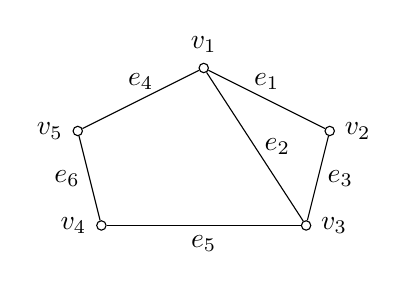
\begin{tikzpicture}[item/.style={circle, draw, fill=white, inner sep=1.2pt}]
				\node[item,label=above:$v_1$] (v1) at (0,2) {};
				\node[item,label=right:$v_2$] (v2) at (1.6,1.2) {};
				\node[item,label=right:$v_3$] (v3) at (1.3,0) {};
				\node[item,label=left:$v_4$]  (v4) at (-1.3,0) {};
				\node[item,label=left:$v_5$]  (v5) at (-1.6,1.2) {};
				\draw (v1)--(v2) node[midway,above] {$e_1$};
				\draw (v1)--(v3) node[midway,right] {$e_2$};
				\draw (v2)--(v3) node[midway,right] {$e_3$};
				\draw (v1)--(v5) node[midway,above] {$e_4$};
				\draw (v3)--(v4) node[midway,below] {$e_5$};
				\draw (v4)--(v5) node[midway,left]  {$e_6$};
			\end{tikzpicture}
		\end{minipage}\hfill
		\begin{minipage}[t]{0.45\textwidth}
			\centering
			\centering
			\small{\textsc{Selection} instance:}\par\vspace{2mm}
			\renewcommand{\arraystretch}{1.1}
			\begin{tabular}{c|ccccc}
				& 1 & 2 & 3 & 4 & 5 \\\hline
				$s_{e_1}$ & 1 & 1 & 0 & 0 & 0 \\
				$s_{e_2}$ & 1 & 0 & 1 & 0 & 0 \\
				$s_{e_3}$ & 0 & 1 & 1 & 0 & 0 \\
				$s_{e_4}$ & 1 & 0 & 0 & 0 & 1 \\
				$s_{e_5}$ & 0 & 0 & 1 & 1 & 0 \\
				$s_{e_6}$ & 0 & 0 & 0 & 1 & 1 \\
			\end{tabular}
		\end{minipage}
	}
	\caption{Reduction from \textsc{Vertex Cover} to \textsc{MaxMin Selection}}
\end{figure}	
	
\section{Computational experiments}
\label{exp}

This chapter presents the empirical evaluation of the approximation algorithms introduced in Chapters~\ref{intro}--\ref{primal-dual}. We begin by outlining the experimental setup, including the instance generation and overarching computational procedures.

All experiments were conducted on a Linux laptop with an AMD Ryzen 5 5625U (12 threads) and 14.5 GiB RAM. All algorithms were implemented in Python~3.12. IPs and LPs were solved using the Gurobi Optimizer~12.0 \cite{gurobi2025}. Numerical computations and data visualizations were performed with NumPy 1.26 and Matplotlib 3.8 \cite{harris2020, hunter2007}.\footnote{All source code required to reproduce the results are openly available in the project's \href{https://github.com/trajana/Approximation_Algorithms_for_the_Robust_Selection_Problem}{GitHub repository}.}

Cost coefficients \( c^s_i\) are drawn independently and uniformly at random from the integer range \([1, 100]\). 
To analyze the isolated impact of each key parameter, we define three configurations in which one parameter is varied explicitly while the others are held fixed or adjusted systematically. 

\begin{itemize}
	\item Config-1 (varying $n$): \( n \in \{2, 4, 6, \dots, 70\} \), \( k = 5 \), \( p = n/2 \).
	
	\item Config-2 (varying $k$): \( n = 20 \), \( k \in \{1, 2, 5, 10, 20, 30, 50, 70, 100\} \), \( p = n/2 = 10 \).
	
	\item Config-3 (varying $p$): \( n = 70 \), \( k = 5 \), \( p \in \{2, 4, \dots, 66, 68\} \).
\end{itemize}

As the central performance metric, we report the empirical approximation ratio, for each instance as
\({\mathrm{ALG}}/{\mathrm{OPT}_{\mathrm{IP}}}\), that is, the objective value of the solution returned by an algorithm divided by the value of an optimal integer solution. For each problem instance, \( m = 100 \) independent runs were conducted.

\begin{figure}[h]
\centering
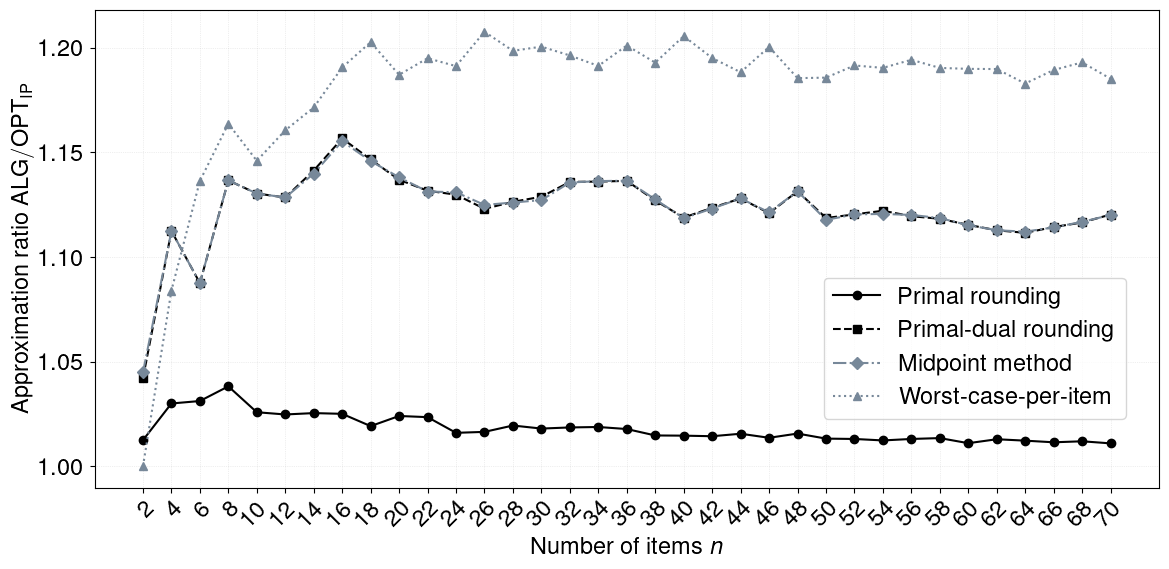
\includegraphics[width=0.9\textwidth]{plot_ratio_comparison_n.png}
\caption{Comparison of approximation ratios in Config-1}\label{config1}
\end{figure}

Figure \ref{config1} shows the behavior of four approximation algorithms as \(n\) grows (Config-1). The primal rounding curve is already close to $1$ for very small $n$ (about $1.02$--$1.03$) and drifts slowly downward as $n$ grows. In contrast, the primal-dual curve and the midpoint method sit around $1.12$--$1.16$ for most $n$, with a better ratio for very small instances (the graphs overlap in the figure).\footnote{In exact arithmetic, primal-dual rounding with fixed weights~$\beta$ selects the $p$ items with smallest weighted costs $w_i$ and thus coincides with the midpoint method (for uniform~$\beta$). In the implementation, floating-point tolerances in the slack tests may treat nearly equal $w_i$ as simultaneously tight, causing different tie-breaking choices. Occasional discrepancies between the two methods are therefore purely numerical.} The wcpi method performs best for \(k=2\), but deteriorates for larger \(n\) (about $1.19$--$1.21$).
Intuitively, primal rounding benefits from the LP's joint view across all scenarios. The primal-dual and midpoint methods, by contrast, rely on average-based scores, and therefore suffer whenever the true worst-case scenario deviates from this average. The wcpi method is optimal for \(n=2\), but overly pessimistic for lager \(n\). 

\begin{figure}[h]
	\centering
	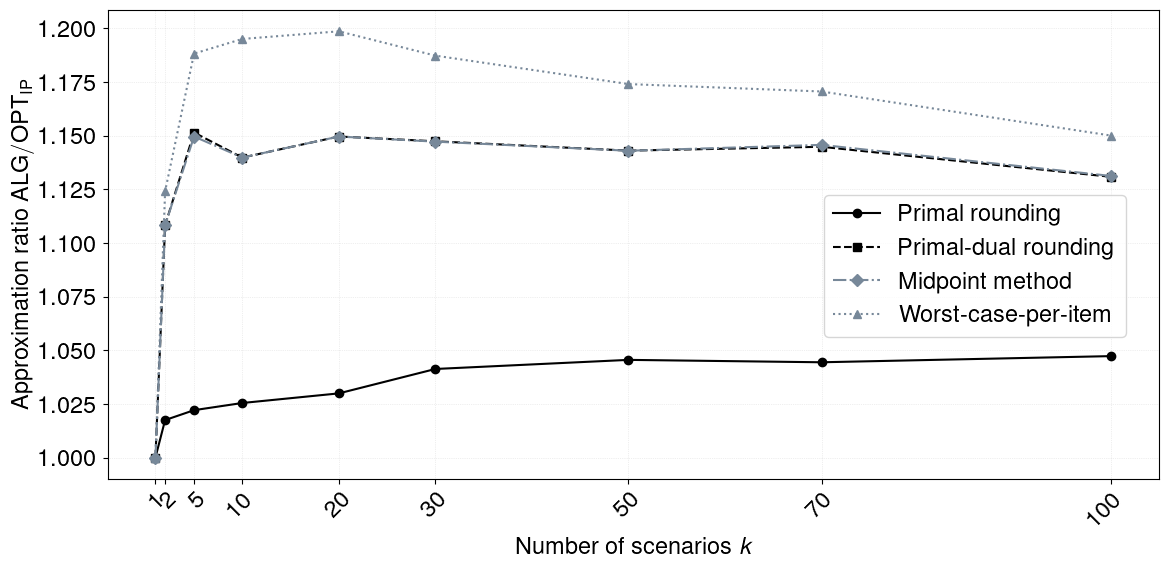
\includegraphics[width=0.9\textwidth]{plot_ratio_comparison_k.png}
	\caption{Comparison of approximation ratios in Config-2}\label{config2}
\end{figure}

Figure \ref{config2} shows sensitivity to the number of scenarios \(k\) (Config-2).
Primal rounding grows from an approximation ratio of $\approx 1.02$ at very small $k$ to about $1.04$--$1.05$ at $k\!=\!100$. Primal-dual rounding and the midpoint method exhibit a sharp jump when moving from $k\!\approx\!2$ to $k\!\approx\!5$ and then plateau at around $1.13$--$1.15$. The wcpi method exhibits a similar behavior with a slightly higher ratio. Consequently, there is a gap between primal rounding and the other methods for $k \ge 5$, which shrinks slightly as \(k\) grows further.  Overall, the methods show a deterioration in solution quality for larger \(k\). This behavior is to be expected, as each additional scenario introduces further conflict into the objective function of the min-max problem, increasing the likelihood of unfavorable cost configurations. 

\begin{figure}[h]
	\centering
	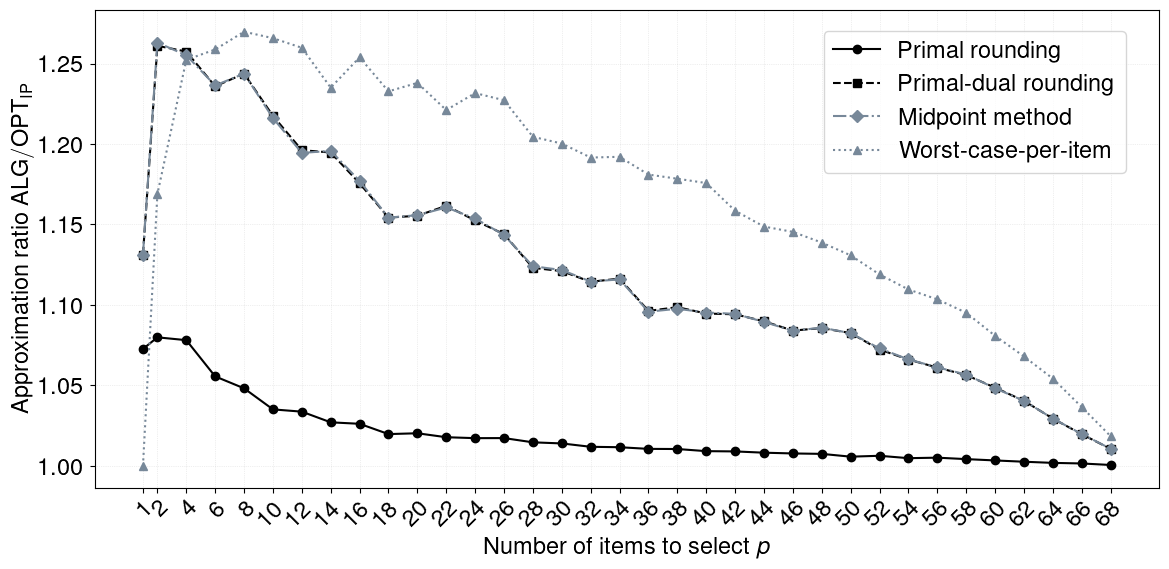
\includegraphics[width=0.9\textwidth]{plot_ratio_comparison_p.png}
	\caption{Comparison of approximation ratios in Config-3}\label{config3}
\end{figure}

Figure~\ref{config3} shows that all algorithms improve with higher values of $p$ and converge toward $1$. However, there is a gap for small $p$. Primal rounding begins near $1.08$ and quickly converges to $\approx1.01$.  Primal-dual rounding and the midpoint method start at around $\approx 1.13$ for $p=1$, shift to $1.25$--$1.27$ for $k=2$ and then decay steadily to $\approx 1.02$ at $p\!=\!68$. The wcpi method shows an interesting behavior, as it is optimal for $p=1$ and almost as good as primal rounding for \(p=2\), but then exhibits a deterioration in solution quality and has the highest approximation ratio of all algorithms for \(p\ge8\).
The overall improvement for growing \(p\) is again expected, since for lager \(p\), the outcome depends on more items, which reduces the impact of any individual rounding discrepancy.

Overall, the experiments show that all four methods exhibit favorable outcomes with approximation ratios consistently close to the optimum and far better than the theoretical bounds. Primal rounding however shows the best empirical results. 

\section{Conclusion}
\label{concl}

Real-world decision making problems are often subject some level of uncertainty. Accounting for these uncertainties tends to increase problem complexity, making approximation algorithms particularly useful in robust optimization. In recent years general approximations for robust combinatorial problems (e.g. midpoint and wcpi) as well as problem specific approximations have been studied intensively.
This paper focuses on the robust \textsc{Selection} problem. The best known approximation for \textsc{MinMax Selection} is based on dependent randomized rounding and provides a tight \(O(\log k/\log\log k)\)-approximation. Despite these existing strong theoretical results, we developed a primal rounding algorithm with a tight bound of \(\min\{k, n - p + 1\}\) improving upon the previous bound whenever \(n-p+1 \;=\; o\!\Big(\frac{\log k}{\log\log k}\Big)\). We also show tightness for the integrality gap \(k\) of our LP. A second algorithm based on primal-dual rounding is presented, which rediscovers and generalizes the midpoint method and exhibits a tight \(k\)-bound. A better approximation can be archived by solving an LP first to find the best representative weight vector. Both algorithms provide a posteriori guarantees. 
Additionally, we give an inapproximability prove for \textsc{MaxMin Selection} for unbounded \(k\).
Our computational experiments indicate that the primal rounding algorithms has the best practical performance. 
These findings indicate that simple rounding schemes are practically effective for the robust \textsc{Selection} problem and that improvements will likely require stronger relaxations or extended formulations.














%
%
%\section{Equations}\label{sec4}
%
%Equations in \LaTeX\ can either be inline or on-a-line by itself (``display equations''). For
%inline equations use the \verb+$...$+ commands. E.g.: The equation
%$H\psi = E \psi$ is written via the command \verb+$H \psi = E \psi$+.
%
%For display equations (with auto generated equation numbers)
%one can use the equation or align environments:
%\begin{equation}
%\|\tilde{X}(k)\|^2 \leq\frac{\sum\limits_{i=1}^{p}\left\|\tilde{Y}_i(k)\right\|^2+\sum\limits_{j=1}^{q}\left\|\tilde{Z}_j(k)\right\|^2 }{p+q}.\label{eq1}
%\end{equation}
%where,
%\begin{align}
%D_\mu &=  \partial_\mu - ig \frac{\lambda^a}{2} A^a_\mu \nonumber \\
%F^a_{\mu\nu} &= \partial_\mu A^a_\nu - \partial_\nu A^a_\mu + g f^{abc} A^b_\mu A^a_\nu \label{eq2}
%\end{align}
%Notice the use of \verb+\nonumber+ in the align environment at the end
%of each line, except the last, so as not to produce equation numbers on
%lines where no equation numbers are required. The \verb+\label{}+ command
%should only be used at the last line of an align environment where
%\verb+\nonumber+ is not used.
%\begin{equation}
%Y_\infty = \left( \frac{m}{\textrm{GeV}} \right)^{-3}
%    \left[ 1 + \frac{3 \ln(m/\textrm{GeV})}{15}
%    + \frac{\ln(c_2/5)}{15} \right]
%\end{equation}
%The class file also supports the use of \verb+\mathbb{}+, \verb+\mathscr{}+ and
%\verb+\mathcal{}+ commands. As such \verb+\mathbb{R}+, \verb+\mathscr{R}+
%and \verb+\mathcal{R}+ produces $\mathbb{R}$, $\mathscr{R}$ and $\mathcal{R}$
%respectively (refer Subsubsection~\ref{subsubsec2}).
%
%\section{Tables}\label{sec5}
%
%Tables can be inserted via the normal table and tabular environment. To put
%footnotes inside tables you should use \verb+\footnotetext[]{...}+ tag.
%The footnote appears just below the table itself (refer Tables~\ref{tab1} and \ref{tab2}). 
%For the corresponding footnotemark use \verb+\footnotemark[...]+
%
%\begin{table}[h]
%\caption{Caption text}\label{tab1}%
%\begin{tabular}{@{}llll@{}}
%\toprule
%Column 1 & Column 2  & Column 3 & Column 4\\
%\midrule
%row 1    & data 1   & data 2  & data 3  \\
%row 2    & data 4   & data 5\footnotemark[1]  & data 6  \\
%row 3    & data 7   & data 8  & data 9\footnotemark[2]  \\
%\botrule
%\end{tabular}
%\footnotetext{Source: This is an example of table footnote. This is an example of table footnote.}
%\footnotetext[1]{Example for a first table footnote. This is an example of table footnote.}
%\footnotetext[2]{Example for a second table footnote. This is an example of table footnote.}
%\end{table}
%
%\noindent
%The input format for the above table is as follows:
%
%%%=============================================%%
%%% For presentation purpose, we have included  %%
%%% \bigskip command. Please ignore this.       %%
%%%=============================================%%
%\bigskip
%\begin{verbatim}
%\begin{table}[<placement-specifier>]
%\caption{<table-caption>}\label{<table-label>}%
%\begin{tabular}{@{}llll@{}}
%\toprule
%Column 1 & Column 2 & Column 3 & Column 4\\
%\midrule
%row 1 & data 1 & data 2	 & data 3 \\
%row 2 & data 4 & data 5\footnotemark[1] & data 6 \\
%row 3 & data 7 & data 8	 & data 9\footnotemark[2]\\
%\botrule
%\end{tabular}
%\footnotetext{Source: This is an example of table footnote. 
%This is an example of table footnote.}
%\footnotetext[1]{Example for a first table footnote.
%This is an example of table footnote.}
%\footnotetext[2]{Example for a second table footnote. 
%This is an example of table footnote.}
%\end{table}
%\end{verbatim}
%\bigskip
%%%=============================================%%
%%% For presentation purpose, we have included  %%
%%% \bigskip command. Please ignore this.       %%
%%%=============================================%%
%
%\begin{table}[h]
%\caption{Example of a lengthy table which is set to full textwidth}\label{tab2}
%\begin{tabular*}{\textwidth}{@{\extracolsep\fill}lcccccc}
%\toprule%
%& \multicolumn{3}{@{}c@{}}{Element 1\footnotemark[1]} & \multicolumn{3}{@{}c@{}}{Element 2\footnotemark[2]} \\\cmidrule{2-4}\cmidrule{5-7}%
%Project & Energy & $\sigma_{calc}$ & $\sigma_{expt}$ & Energy & $\sigma_{calc}$ & $\sigma_{expt}$ \\
%\midrule
%Element 3  & 990 A & 1168 & $1547\pm12$ & 780 A & 1166 & $1239\pm100$\\
%Element 4  & 500 A & 961  & $922\pm10$  & 900 A & 1268 & $1092\pm40$\\
%\botrule
%\end{tabular*}
%\footnotetext{Note: This is an example of table footnote. This is an example of table footnote this is an example of table footnote this is an example of~table footnote this is an example of table footnote.}
%\footnotetext[1]{Example for a first table footnote.}
%\footnotetext[2]{Example for a second table footnote.}
%\end{table}
%
%In case of double column layout, tables which do not fit in single column width should be set to full text width. For this, you need to use \verb+\begin{table*}+ \verb+...+ \verb+\end{table*}+ instead of \verb+\begin{table}+ \verb+...+ \verb+\end{table}+ environment. Lengthy tables which do not fit in textwidth should be set as rotated table. For this, you need to use \verb+\begin{sidewaystable}+ \verb+...+ \verb+\end{sidewaystable}+ instead of \verb+\begin{table*}+ \verb+...+ \verb+\end{table*}+ environment. This environment puts tables rotated to single column width. For tables rotated to double column width, use \verb+\begin{sidewaystable*}+ \verb+...+ \verb+\end{sidewaystable*}+.
%
%\begin{sidewaystable}
%\caption{Tables which are too long to fit, should be written using the ``sidewaystable'' environment as shown here}\label{tab3}
%\begin{tabular*}{\textheight}{@{\extracolsep\fill}lcccccc}
%\toprule%
%& \multicolumn{3}{@{}c@{}}{Element 1\footnotemark[1]}& \multicolumn{3}{@{}c@{}}{Element\footnotemark[2]} \\\cmidrule{2-4}\cmidrule{5-7}%
%Projectile & Energy	& $\sigma_{calc}$ & $\sigma_{expt}$ & Energy & $\sigma_{calc}$ & $\sigma_{expt}$ \\
%\midrule
%Element 3 & 990 A & 1168 & $1547\pm12$ & 780 A & 1166 & $1239\pm100$ \\
%Element 4 & 500 A & 961  & $922\pm10$  & 900 A & 1268 & $1092\pm40$ \\
%Element 5 & 990 A & 1168 & $1547\pm12$ & 780 A & 1166 & $1239\pm100$ \\
%Element 6 & 500 A & 961  & $922\pm10$  & 900 A & 1268 & $1092\pm40$ \\
%\botrule
%\end{tabular*}
%\footnotetext{Note: This is an example of table footnote this is an example of table footnote this is an example of table footnote this is an example of~table footnote this is an example of table footnote.}
%\footnotetext[1]{This is an example of table footnote.}
%\end{sidewaystable}
%
%\section{Figures}\label{sec6}
%
%As per the \LaTeX\ standards you need to use eps images for \LaTeX\ compilation and \verb+pdf/jpg/png+ images for \verb+PDFLaTeX+ compilation. This is one of the major difference between \LaTeX\ and \verb+PDFLaTeX+. Each image should be from a single input .eps/vector image file. Avoid using subfigures. The command for inserting images for \LaTeX\ and \verb+PDFLaTeX+ can be generalized. The package used to insert images in \verb+LaTeX/PDFLaTeX+ is the graphicx package. Figures can be inserted via the normal figure environment as shown in the below example:
%
%%%=============================================%%
%%% For presentation purpose, we have included  %%
%%% \bigskip command. Please ignore this.       %%
%%%=============================================%%
%\bigskip
%\begin{verbatim}
%\begin{figure}[<placement-specifier>]
%\centering
%\includegraphics{<eps-file>}
%\caption{<figure-caption>}\label{<figure-label>}
%\end{figure}
%\end{verbatim}
%\bigskip
%%%=============================================%%
%%% For presentation purpose, we have included  %%
%%% \bigskip command. Please ignore this.       %%
%%%=============================================%%
%
%\begin{figure}[h]
%\centering
%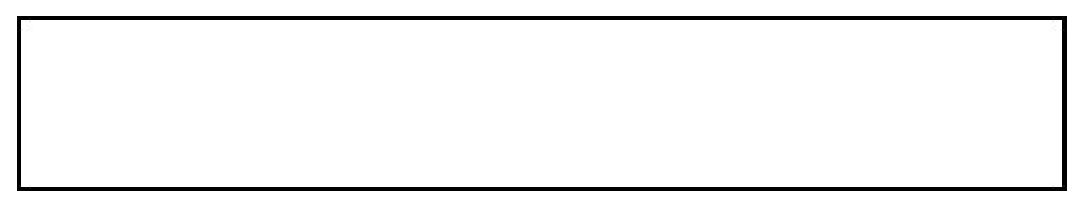
\includegraphics[width=0.9\textwidth]{fig.eps}
%\caption{This is a widefig. This is an example of long caption this is an example of long caption  this is an example of long caption this is an example of long caption}\label{fig1}
%\end{figure}
%
%In case of double column layout, the above format puts figure captions/images to single column width. To get spanned images, we need to provide \verb+\begin{figure*}+ \verb+...+ \verb+\end{figure*}+.
%
%For sample purpose, we have included the width of images in the optional argument of \verb+\includegraphics+ tag. Please ignore this. 
%
%\section{Algorithms, Program codes and Listings}\label{sec7}
%
%Packages \verb+algorithm+, \verb+algorithmicx+ and \verb+algpseudocode+ are used for setting algorithms in \LaTeX\ using the format:
%
%%%=============================================%%
%%% For presentation purpose, we have included  %%
%%% \bigskip command. Please ignore this.       %%
%%%=============================================%%
%\bigskip
%\begin{verbatim}
%\begin{algorithm}
%\caption{<alg-caption>}\label{<alg-label>}
%\begin{algorithmic}[1]
%. . .
%\end{algorithmic}
%\end{algorithm}
%\end{verbatim}
%\bigskip
%%%=============================================%%
%%% For presentation purpose, we have included  %%
%%% \bigskip command. Please ignore this.       %%
%%%=============================================%%
%
%You may refer above listed package documentations for more details before setting \verb+algorithm+ environment. For program codes, the ``verbatim'' package is required and the command to be used is \verb+\begin{verbatim}+ \verb+...+ \verb+\end{verbatim}+. 
%
%Similarly, for \verb+listings+, use the \verb+listings+ package. \verb+\begin{lstlisting}+ \verb+...+ \verb+\end{lstlisting}+ is used to set environments similar to \verb+verbatim+ environment. Refer to the \verb+lstlisting+ package documentation for more details.
%
%A fast exponentiation procedure:
%
%\lstset{texcl=true,basicstyle=\small\sf,commentstyle=\small\rm,mathescape=true,escapeinside={(*}{*)}}
%\begin{lstlisting}
%begin
%  for $i:=1$ to $10$ step $1$ do
%      expt($2,i$);  
%      newline() od                (*\textrm{Comments will be set flush to the right margin}*)
%where
%proc expt($x,n$) $\equiv$
%  $z:=1$;
%  do if $n=0$ then exit fi;
%     do if odd($n$) then exit fi;                 
%        comment: (*\textrm{This is a comment statement;}*)
%        $n:=n/2$; $x:=x*x$ od;
%     { $n>0$ };
%     $n:=n-1$; $z:=z*x$ od;
%  print($z$). 
%end
%\end{lstlisting}
%
%\begin{algorithm}
%\caption{Calculate $y = x^n$}\label{algo1}
%\begin{algorithmic}[1]
%\Require $n \geq 0 \vee x \neq 0$
%\Ensure $y = x^n$ 
%\State $y \Leftarrow 1$
%\If{$n < 0$}\label{algln2}
%        \State $X \Leftarrow 1 / x$
%        \State $N \Leftarrow -n$
%\Else
%        \State $X \Leftarrow x$
%        \State $N \Leftarrow n$
%\EndIf
%\While{$N \neq 0$}
%        \If{$N$ is even}
%            \State $X \Leftarrow X \times X$
%            \State $N \Leftarrow N / 2$
%        \Else[$N$ is odd]
%            \State $y \Leftarrow y \times X$
%            \State $N \Leftarrow N - 1$
%        \EndIf
%\EndWhile
%\end{algorithmic}
%\end{algorithm}
%
%%%=============================================%%
%%% For presentation purpose, we have included  %%
%%% \bigskip command. Please ignore this.       %%
%%%=============================================%%
%\bigskip
%\begin{minipage}{\hsize}%
%\lstset{frame=single,framexleftmargin=-1pt,framexrightmargin=-17pt,framesep=12pt,linewidth=0.98\textwidth,language=pascal}% Set your language (you can change the language for each code-block optionally)
%%%% Start your code-block
%\begin{lstlisting}
%for i:=maxint to 0 do
%begin
%{ do nothing }
%end;
%Write('Case insensitive ');
%Write('Pascal keywords.');
%\end{lstlisting}
%\end{minipage}
%
%\section{Cross referencing}\label{sec8}
%
%Environments such as figure, table, equation and align can have a label
%declared via the \verb+\label{#label}+ command. For figures and table
%environments use the \verb+\label{}+ command inside or just
%below the \verb+\caption{}+ command. You can then use the
%\verb+\ref{#label}+ command to cross-reference them. As an example, consider
%the label declared for Figure~\ref{fig1} which is
%\verb+\label{fig1}+. To cross-reference it, use the command 
%\verb+Figure \ref{fig1}+, for which it comes up as
%``Figure~\ref{fig1}''. 
%
%To reference line numbers in an algorithm, consider the label declared for the line number 2 of Algorithm~\ref{algo1} is \verb+\label{algln2}+. To cross-reference it, use the command \verb+\ref{algln2}+ for which it comes up as line~\ref{algln2} of Algorithm~\ref{algo1}.
%
%\subsection{Details on reference citations}\label{subsec7}
%
%Standard \LaTeX\ permits only numerical citations. To support both numerical and author-year citations this template uses \verb+natbib+ \LaTeX\ package. For style guidance please refer to the template user manual.
%
%Here is an example for \verb+\cite{...}+: \cite{bib1}. Another example for \verb+\citep{...}+: \citep{bib2}. For author-year citation mode, \verb+\cite{...}+ prints Jones et al. (1990) and \verb+\citep{...}+ prints (Jones et al., 1990).
%
%All cited bib entries are printed at the end of this article: \cite{bib3}, \cite{bib4}, \cite{bib5}, \cite{bib6}, \cite{bib7}, \cite{bib8}, \cite{bib9}, \cite{bib10}, \cite{bib11}, \cite{bib12} and \cite{bib13}.
%
%\section{Examples for theorem like environments}\label{sec10}
%
%For theorem like environments, we require \verb+amsthm+ package. There are three types of predefined theorem styles exists---\verb+thmstyleone+, \verb+thmstyletwo+ and \verb+thmstylethree+ 
%
%%%=============================================%%
%%% For presentation purpose, we have included  %%
%%% \bigskip command. Please ignore this.       %%
%%%=============================================%%
%\bigskip
%\begin{tabular}{|l|p{19pc}|}
%\hline
%\verb+thmstyleone+ & Numbered, theorem head in bold font and theorem text in italic style \\\hline
%\verb+thmstyletwo+ & Numbered, theorem head in roman font and theorem text in italic style \\\hline
%\verb+thmstylethree+ & Numbered, theorem head in bold font and theorem text in roman style \\\hline
%\end{tabular}
%\bigskip
%%%=============================================%%
%%% For presentation purpose, we have included  %%
%%% \bigskip command. Please ignore this.       %%
%%%=============================================%%
%
%For mathematics journals, theorem styles can be included as shown in the following examples:
%
%\begin{theorem}[Theorem subhead]\label{thm1}
%Example theorem text. Example theorem text. Example theorem text. Example theorem text. Example theorem text. 
%Example theorem text. Example theorem text. Example theorem text. Example theorem text. Example theorem text. 
%Example theorem text. 
%\end{theorem}
%
%Sample body text. Sample body text. Sample body text. Sample body text. Sample body text. Sample body text. Sample body text. Sample body text.
%
%\begin{proposition}
%Example proposition text. Example proposition text. Example proposition text. Example proposition text. Example proposition text. 
%Example proposition text. Example proposition text. Example proposition text. Example proposition text. Example proposition text. 
%\end{proposition}
%
%Sample body text. Sample body text. Sample body text. Sample body text. Sample body text. Sample body text. Sample body text. Sample body text.
%
%\begin{example}
%Phasellus adipiscing semper elit. Proin fermentum massa
%ac quam. Sed diam turpis, molestie vitae, placerat a, molestie nec, leo. Maecenas lacinia. Nam ipsum ligula, eleifend
%at, accumsan nec, suscipit a, ipsum. Morbi blandit ligula feugiat magna. Nunc eleifend consequat lorem. 
%\end{example}
%
%Sample body text. Sample body text. Sample body text. Sample body text. Sample body text. Sample body text. Sample body text. Sample body text.
%
%\begin{remark}
%Phasellus adipiscing semper elit. Proin fermentum massa
%ac quam. Sed diam turpis, molestie vitae, placerat a, molestie nec, leo. Maecenas lacinia. Nam ipsum ligula, eleifend
%at, accumsan nec, suscipit a, ipsum. Morbi blandit ligula feugiat magna. Nunc eleifend consequat lorem. 
%\end{remark}
%
%Sample body text. Sample body text. Sample body text. Sample body text. Sample body text. Sample body text. Sample body text. Sample body text.
%
%\begin{definition}[Definition sub head]
%Example definition text. Example definition text. Example definition text. Example definition text. Example definition text. Example definition text. Example definition text. Example definition text. 
%\end{definition}
%
%Additionally a predefined ``proof'' environment is available: \verb+\begin{proof}+ \verb+...+ \verb+\end{proof}+. This prints a ``Proof'' head in italic font style and the ``body text'' in roman font style with an open square at the end of each proof environment. 
%
%\begin{proof}
%Example for proof text. Example for proof text. Example for proof text. Example for proof text. Example for proof text. Example for proof text. Example for proof text. Example for proof text. Example for proof text. Example for proof text. 
%\end{proof}
%
%Sample body text. Sample body text. Sample body text. Sample body text. Sample body text. Sample body text. Sample body text. Sample body text.
%
%\begin{proof}[Proof of Theorem~{\upshape\ref{thm1}}]
%Example for proof text. Example for proof text. Example for proof text. Example for proof text. Example for proof text. Example for proof text. Example for proof text. Example for proof text. Example for proof text. Example for proof text. 
%\end{proof}
%
%\noindent
%For a quote environment, use \verb+\begin{quote}...\end{quote}+
%\begin{quote}
%Quoted text example. Aliquam porttitor quam a lacus. Praesent vel arcu ut tortor cursus volutpat. In vitae pede quis diam bibendum placerat. Fusce elementum
%convallis neque. Sed dolor orci, scelerisque ac, dapibus nec, ultricies ut, mi. Duis nec dui quis leo sagittis commodo.
%\end{quote}
%
%Sample body text. Sample body text. Sample body text. Sample body text. Sample body text (refer Figure~\ref{fig1}). Sample body text. Sample body text. Sample body text (refer Table~\ref{tab3}). 
%
%\section{Methods}\label{sec11}
%
%Topical subheadings are allowed. Authors must ensure that their Methods section includes adequate experimental and characterization data necessary for others in the field to reproduce their work. Authors are encouraged to include RIIDs where appropriate. 
%
%\textbf{Ethical approval declarations} (only required where applicable) Any article reporting experiment/s carried out on (i)~live vertebrate (or higher invertebrates), (ii)~humans or (iii)~human samples must include an unambiguous statement within the methods section that meets the following requirements: 
%
%\begin{enumerate}[1.]
%\item Approval: a statement which confirms that all experimental protocols were approved by a named institutional and/or licensing committee. Please identify the approving body in the methods section
%
%\item Accordance: a statement explicitly saying that the methods were carried out in accordance with the relevant guidelines and regulations
%
%\item Informed consent (for experiments involving humans or human tissue samples): include a statement confirming that informed consent was obtained from all participants and/or their legal guardian/s
%\end{enumerate}
%
%If your manuscript includes potentially identifying patient/participant information, or if it describes human transplantation research, or if it reports results of a clinical trial then  additional information will be required. Please visit (\url{https://www.nature.com/nature-research/editorial-policies}) for Nature Portfolio journals, (\url{https://www.springer.com/gp/authors-editors/journal-author/journal-author-helpdesk/publishing-ethics/14214}) for Springer Nature journals, or (\url{https://www.biomedcentral.com/getpublished/editorial-policies\#ethics+and+consent}) for BMC.
%
%\section{Discussion}\label{sec12}
%
%Discussions should be brief and focused. In some disciplines use of Discussion or `Conclusion' is interchangeable. It is not mandatory to use both. Some journals prefer a section `Results and Discussion' followed by a section `Conclusion'. Please refer to Journal-level guidance for any specific requirements. 
%
%\section{Conclusion}\label{sec13}
%
%Conclusions may be used to restate your hypothesis or research question, restate your major findings, explain the relevance and the added value of your work, highlight any limitations of your study, describe future directions for research and recommendations. 
%
%In some disciplines use of Discussion or 'Conclusion' is interchangeable. It is not mandatory to use both. Please refer to Journal-level guidance for any specific requirements. 
%
%\backmatter
%
%\bmhead{Supplementary information}
%
%If your article has accompanying supplementary file/s please state so here. 
%
%Authors reporting data from electrophoretic gels and blots should supply the full unprocessed scans for key as part of their Supplementary information. This may be requested by the editorial team/s if it is missing.
%
%Please refer to Journal-level guidance for any specific requirements.
%
%\bmhead{Acknowledgements}
%
%Acknowledgements are not compulsory. Where included they should be brief. Grant or contribution numbers may be acknowledged.
%
%Please refer to Journal-level guidance for any specific requirements.
%
%\section*{Declaration}
%
%The authors have no relevant financial or non-financial interests to disclose.
%
%%%===================================================%%
%%% For presentation purpose, we have included        %%
%%% \bigskip command. Please ignore this.             %%
%%%===================================================%%
%\bigskip
%\begin{flushleft}%
%Editorial Policies for:
%
%\bigskip\noindent
%Springer journals and proceedings: \url{https://www.springer.com/gp/editorial-policies}
%\end{flushleft}
%
%\begin{appendices}
%
%\section{Tightness of primal rounding}\label{primal_tight}
%
%
%
%\end{appendices}

%%===========================================================================================%%
%% If you are submitting to one of the Nature Portfolio journals, using the eJP submission   %%
%% system, please include the references within the manuscript file itself. You may do this  %%
%% by copying the reference list from your .bbl file, paste it into the main manuscript .tex %%
%% file, and delete the associated \verb+\bibliography+ commands.                            %%
%%===========================================================================================%%

\bibliography{sn-bibliography}% common bib file
%% if required, the content of .bbl file can be included here once bbl is generated
%%\input sn-article.bbl

\end{document}
